\documentclass[letterpaper,12pt]{article}

% --- PAQUETES DE IDIOMA
\usepackage[spanish,mexico]{babel}
\addto\captionsspanish{\renewcommand{\contentsname}{Indice}}
\usepackage[utf8]{inputenc}
\usepackage{csquotes}
\usepackage{iftex}

\usepackage{pdfpages}

% --- PAQUETES MATEMÁTICOS --
\usepackage{amsmath}
\usepackage{cancel}
\usepackage{mathrsfs}

% --- PAQUETES GRÁFICOS Y DE DISEÑO ---
\usepackage{graphicx}
\usepackage{float}
\usepackage{placeins}
\usepackage{needspace}
\usepackage{subcaption}
\usepackage[table]{xcolor}
\usepackage{makecell}
\usepackage{array}
\usepackage{tikz}
\usetikzlibrary{shapes.geometric, shapes.multipart, positioning, arrows.meta, calc, shadows, decorations.pathreplacing,babel}

% --- LISTAS ---
\usepackage{enumitem}

% --- PAQUETES DE CÓDIGO ---
\usepackage{listings}
% Configuración del estilo de listings
\definecolor{codebg}{rgb}{0.95,0.95,0.95}   
\definecolor{keyword}{rgb}{0.0,0.2,0.6}     
\definecolor{comment}{rgb}{0.25,0.5,0.35}   
\definecolor{string}{rgb}{0.6,0.0,0.0}      
\definecolor{number}{rgb}{0.5,0.0,0.5}      
\definecolor{codegray}{rgb}{0.5,0.5,0.5}
\definecolor{codepurple}{rgb}{0.58,0,0.82}
\definecolor{backcolour}{rgb}{0.95,0.95,0.95}

\lstset{
  backgroundcolor=\color{backcolour},
  basicstyle=\ttfamily\small,
  keywordstyle=\color{blue}\bfseries,
  stringstyle=\color{codepurple},
  commentstyle=\color{codegray}\itshape,
  numbers=left,
  numberstyle=\tiny\color{codegray},
  frame=single,
  rulecolor=\color{black},
  breaklines=true,
  tabsize=4,
  showstringspaces=false,
  literate={á}{{\'a}}1
           {é}{{\'e}}1
           {í}{{\'i}}1
           {ó}{{\'o}}1
           {ú}{{\'u}}1
           {Á}{{\'A}}1
           {É}{{\'E}}1
           {Í}{{\'I}}1
           {Ó}{{\'O}}1
           {Ú}{{\'U}}1
           {ñ}{{\~n}}1
           {Ñ}{{\~N}}1
           {¿}{{\textquestiondown}}1
           {¡}{{\textexclamdown}}1
}


% Estilo para código en C
\lstdefinestyle{cstyle}{
  language=C,
  backgroundcolor=\color{backcolour},
  basicstyle=\ttfamily\small,
  keywordstyle=\color{blue}\bfseries,
    keywordstyle=[2]\color{yellow!70!orange}\bfseries,
    morekeywords=[2]{MPI_Init,MPI_Comm_size,MPI_Comm_rank,MPI_Send,MPI_Recv,MPI_Scatter,MPI_Gather,MPI_Bcast,MPI_Reduce,MPI_Finalize},
    emph={printf},
    emphstyle=\color{blue}\bfseries,
  stringstyle=\color{codepurple},
  commentstyle=\color{codegray}\itshape,
  numbers=left,
  numberstyle=\tiny\color{codegray},
  frame=single,
  rulecolor=\color{black},
  breaklines=true,
  tabsize=4,
  showstringspaces=false
}

% Definición del lenguaje Python para listings
\lstdefinelanguage[LAB]{Python}{
    morekeywords={False, None, True, and, as, assert, async, await, break,
                                class, continue, def, del, elif, else, except, finally,
                                for, from, global, if, import, in, is, lambda, nonlocal,
                                not, or, pass, raise, return, try, while, with, yield,
                                machine, Pin, PWM, ADC, Timer, sleep_ms, sleep_us},
    morecomment=[l]{\#},
    morestring=[b]",
    morestring=[b]',
    sensitive=true
}

% Estilo para salidas de consola/terminal
\lstdefinestyle{output}{
  backgroundcolor=\color{black!5},
  basicstyle=\ttfamily\footnotesize,
  numbers=none,
  frame=single,
  rulecolor=\color{black!30},
  breaklines=true,
  tabsize=4,
  showstringspaces=false,
  xleftmargin=0.5cm,
  xrightmargin=0.5cm
}

% --- ESTILOS PARA DIAGRAMAS DE FLUJO (TIKZ) ---
\tikzset{
  startstop/.style={rectangle, rounded corners, minimum width=3cm, minimum height=1cm,text centered, draw=black, fill=red!30},
  process/.style={rectangle, minimum width=3cm, minimum height=1cm, text centered, draw=black, fill=orange!30},
  decision/.style={diamond, aspect=2, minimum width=3cm, minimum height=1cm, text centered, draw=black, fill=green!30},
  io/.style={trapezium, trapezium left angle=70, trapezium right angle=110, minimum width=3cm, minimum height=1cm, text centered, draw=black, fill=blue!30},
  arrow/.style={thick,->,>=stealth}
}


\definecolor{azulresultado}{HTML}{0072C6}
\definecolor{rojoacarreo}{HTML}{FF0000}

% --- RUTAS DE IMÁGENES ---
\graphicspath{{img/}{portada_img/}}

\definecolor{armblue}{RGB}{0, 113, 188}

% --- ÍNDICE CON PUNTOS ---
\usepackage{tocloft}
\renewcommand{\cftsecleader}{\cftdotfill{\cftdotsep}}

% --- CONFIGURACIÓN DE PÁGINA (GEOMETRÍA) ---
\usepackage[
    left=25mm, 
    right=25mm,
    top=35mm,
    bottom=30mm,
    headheight=77pt, 
    papersize={21.59cm,27.94cm}
]{geometry}

% --- FORMATO DE TEXTO ---
\usepackage{setspace}
\onehalfspacing
\usepackage{parskip} 
\usepackage{lipsum}  

% --- VARIABLES GLOBALES ---
\newcommand{\materia}{}

% --- ENCABEZADOS Y PIES DE PÁGINA ---
\usepackage{fancyhdr}
\pagestyle{fancy}
\fancyhf{} 
\fancyhead[L]{
\includegraphics[height=1.5cm]{portada_img/der.png}}
\fancyhead[R]{
\includegraphics[height=1.5cm]{portada_img/izq.png}}
\fancyfoot[C]{\thepage} 

\renewcommand{\headrulewidth}{0.4pt} 
\renewcommand{\footrulewidth}{0pt}  

% --- BIBLIOGRAFÍA ---
\usepackage[backend=biber, style=apa, sortcites, url=true]{biblatex}
\addbibresource{referencias.bib}

% --- HIPERVÍNCULOS ---
\usepackage{hyperref}
\hypersetup{
    colorlinks=true,
    linkcolor=blue,
    citecolor=blue,
    filecolor=magenta,
    urlcolor=cyan
}


\fancypagestyle{estiloindice}{
  \fancyhf{} 
  \fancyhead[L]{
\includegraphics[height=1.5cm]{portada_img/der.png}}
  \fancyhead[R]{
\includegraphics[height=1.5cm]{portada_img/izq.png}}
  \renewcommand{\headrulewidth}{0.4pt} 
  \renewcommand{\footrulewidth}{0pt}
}

\begin{document}
\setlength{\emergencystretch}{1em}
\hypersetup{pageanchor=false}
\thispagestyle{empty} % Sin encabezado ni pie en la portada

% --- ENCABEZADO DE PORTADA (TABLA DE 3 COLUMNAS) ---
\begin{center}
    % La tabla usa 'm' para centrar verticalmente las imagenes y el texto
    \begin{tabular}{m{0.15\textwidth} m{0.60\textwidth} m{0.15\textwidth}}
        % Logo Izquierdo (UNAM)
        
\includegraphics[width=2cm]{portada_img/der.png} & 
        
        % Titulo Central
        \centering\Huge\textbf{Universidad Nacional Autonoma de Mexico} &
        
        % Logo Derecho (Facultad)
        \raggedleft
\includegraphics[width=2cm]{portada_img/izq.png}
    \end{tabular}
\end{center}

\vspace{0.3cm}

% --- INFORMACION DEL REPORTE ---
\begin{center}
    {\LARGE \textbf{Facultad de Ingenieria}}\\[1cm]

    {\LARGE \textbf{Alumno:}}\\[0.3cm]
    {\Large Lara Hernandez Angel Husiel - 320060829} \\[1cm]


    {\LARGE \textbf{Seguridad informatica basica}} \\[1cm]
    {\LARGE \textbf{Grupo:} 4 } \\[1cm]

	{\LARGE Semestre: 2027-1} \\[1cm]
    
    {\LARGE \textbf{Tarea 3}}\\[0.5cm]

    {\LARGE {ATT\&CKcon 7.0}}\\[1cm]


    {\Large \textbf{Fecha de Entrega:}}\\[0.2cm]
    {\Large 31 de Octubre del 2026}
\end{center}
\newpage
{\hypersetup{linkcolor=black}\tableofcontents}
\thispagestyle{estiloindice}
\newpage
\thispagestyle{fancy}
\setcounter{page}{1}
\hypersetup{pageanchor=true}
\singlespacing

\section{Charlas asistidas}

Las charlas asistidas asistidias, fueron del dia 27 de octubre, siendo del primer dia 
de las conferencias, asistiendo desde las 9 de la mañana hasta las 3 de la tarde.

Para esto, se tuvieron 6 platicas, en las cuales entre medio de la 3 y 4, hubo un breve
descanso.

Las seis charlas son las siguientes: 

\begin{enumerate}
    \item Obfuscated Tale: From ATT\&CK Origin to Detection Today.
    \item Multi-Tenant Kill Chain Correlation: ATT\&CK-Stage Progression Scoring Across Identities and Organizations in SaaS Environments.
    \item The Defensible Minimum: Threat-Informed Defense When You Can't Afford the Matrix.
    \item MITRE ATT\&CK Updates: Enterprise ATT\&CK.
    \item Measuring ATT\&CK Coverage Through Real Malware Tradecraft: Beyond T1055.
    \item Breaking the Defenders: Measuring Defense Impairment at Scale Through MSP Telemetry.
\end{enumerate}

En general, algo que se repitio en las distintas ponencias fue
que tener una tecnica marcada en una matriz no demuestra que
realmente se pueda detectar. Esto me parecio importante por que
en las practicas hemos identificado las acciones que se realizan
durante un ataque, pero aqui se mostro que tambien se tiene que
comprobar que informacion recibe el defensor y que puede hacer
con ella.

\section{Experiencia personal y presentaciones}

\subsection{Obfuscated Tale: From ATT\&CK Origin to Detection Today}

Empezo con la explicacion de que los atacantes pueden
cambiar la forma en la que escriben o preparan un archivo,
mientras que varias de las acciones que necesitan realizar siguen
siendo parecidas. 

Para esto, se mencionaron ejemplos con PowerShell, contenido
codificado en Base64, para este caso, se nos explico que en el caso 
de Base64 sirve para
representar informacion mediante otra codificacion y gzip para
comprimirla.

Ahora bien, el punto que me parecio mas importante fue la
diferencia entre registrar una accion y detectarla. Se puede
tener el comando dentro de algun archivo, esto empezo siendo la 
parte principal, para poder ver desde donde inicia el ataque y aun asi no
generar una alerta, por que todavia falta una regla que
interprete lo que paso. Es donde entro el otro 
tema a hablar, que fue el caso de la telemetria, que
son los datos que se recolectan sobre la actividad del sistema,
como los procesos que se crean, los scripts que se ejecutan y las
conexiones que se realizan.

Despues de esto, se explico el uso de los eventos 4104 y 4103 de
PowerShell, relacionados con el registro de bloques de script y
de modulos. Tambien se menciono Sysmon, donde el evento 1 permite
revisar la creacion de procesos, el 7 la carga de imagenes,
incluyendo DLL, y el 17 la creacion de tuberias con nombre. Lo
que se busca es relacionar los eventos para entender que programa
inicio a otro y con que argumentos.


\begin{figure}[H]
    \centering
    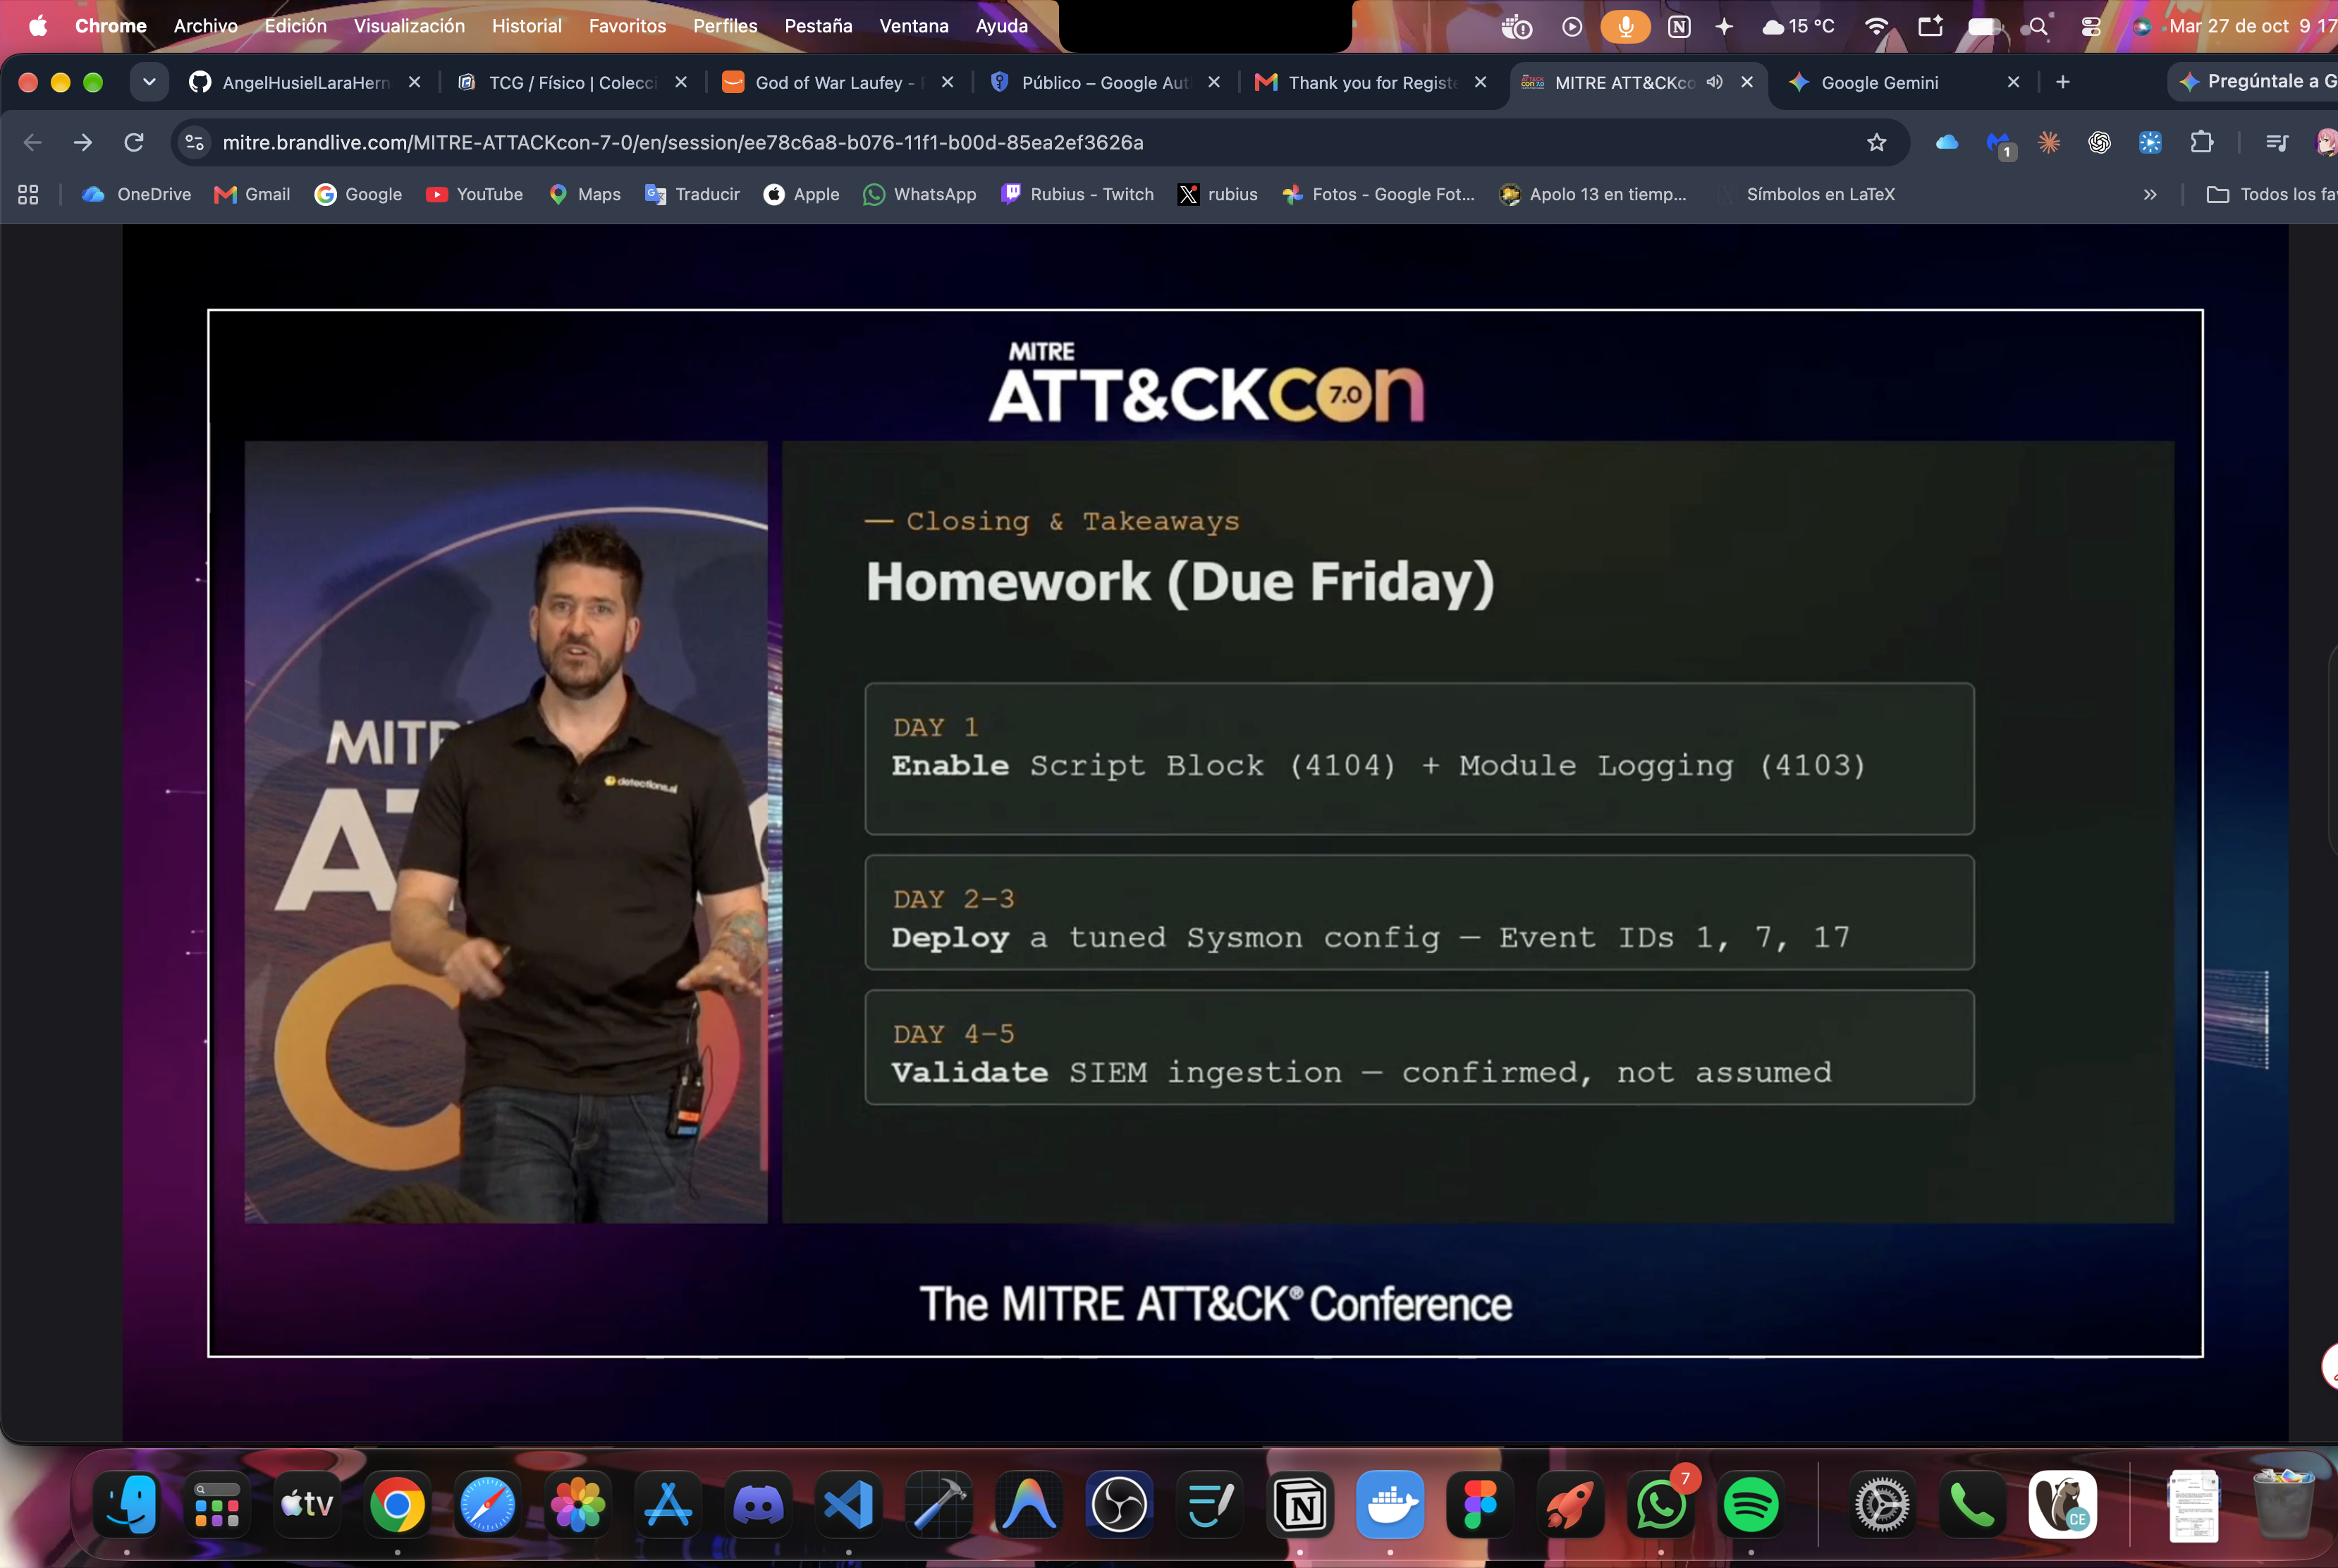
\includegraphics[width=\textwidth,trim=145.01bp 97.00bp 73.00bp 215.01bp,clip]{img/image3.png}
    \caption{Recomendaciones sobre registros de PowerShell, Sysmon y validacion de la recepcion en el SIEM.}
\end{figure}

Elementos a destacar:

\begin{itemize}
    \item Diferenciar entre tener un evento registrado y tener una deteccion que lo utilice.
    \item Revisar la relacion entre los procesos y no solamente una palabra dentro del comando.
    \item Comprobar que los registros realmente llegan al SIEM, que es la plataforma que permite reunirlos y analizarlos.
\end{itemize}

\Needspace{10\baselineskip}
\subsection{Multi-Tenant Kill Chain Correlation en entornos SaaS}

En esta segunda presentacion se hablo de un problema distinto,
pero relacionado con la misma idea: una alerta puede parecer poco
importante si se revisa sola, mientras que al relacionarla con
otras acciones puede mostrar una cadena de conexiones, lo que hace que 
sea tanto mas peligrosa, como se revele el patron de comportamiento 
de algun atacante o de los ataques. Se uso de ejemplo un SaaS, 
que son aplicaciones que se
utilizan como un servicio.

Donde un tenant es el entorno de una organizacion dentro del
servicio. La propuesta consistio en relacionar los eventos de una
misma identidad a lo largo de un periodo y darles contexto segun
las etapas de ATT\&CK. Para esto, se trato como punto principal
revisar si las acciones tenian una relacion
que ayudara a explicar lo que estaba ocurriendo.

Algo a recalcar fue la diferencia entre una anomalia y una accion
concreta. Por ejemplo, cambiar de proveedor de internet o de
identificador del navegador puede ser algo extraño, pero no
demuestra por si solo que una cuenta fue comprometida. Por otro
lado, reutilizar un token de acceso, modificar la configuracion
de autenticacion o cambiar una regla del correo son acciones que
aportan otro tipo de evidencia. La anomalia ayuda a interpretar
el caso, pero no debe reemplazar esa evidencia.

En lo personal, la parte que mas me intereso fue la correlacion
entre organizaciones. Una integracion o una aplicacion de
terceros puede tocar varios entornos, por lo que una secuencia de
intentos fallidos en una sola empresa no siempre cuenta toda la
historia. Si se encuentra el mismo patron en varios entornos y se
relaciona con una identidad de integracion compartida, se puede
ampliar la investigacion. Esto no significa que compartir una IP
sea suficiente para afirmar que existe un ataque.

Elementos a destacar:

\begin{itemize}
    \item Usar las etapas de ATT\&CK para relacionar acciones de una misma identidad.
    \item Distinguir el contexto de una anomalia de la evidencia concreta de una accion.
    \item Combinar la correlacion entre organizaciones con las reglas y el conocimiento de los analistas.
\end{itemize}

\Needspace{10\baselineskip}
\subsection{The Defensible Minimum}

El problema que
planteo fue que no todas las organizaciones pueden mantener un
centro de operaciones de seguridad completo, una herramienta en
cada equipo y todos los registros que se quisieran tener.

Ahora bien, lo que me parecio importante fue que no se presento
esto como una razon para dejar de defenderse. Se propuso
identificar un minimo defendible, donde se toma lo que es
importante para las amenazas de la organizacion y se compara con
lo que realmente se puede implementar, mantener y comprobar. Lo
que queda fuera se tiene que reconocer como riesgo pendiente, en
lugar de marcarlo como cubierto solamente por que aparece en una
herramienta.

En lo personal, esto me hizo sentido con las practicas. Nosotros
trabajamos con maquinas y herramientas especificas, por lo que
cada resultado depende de lo que se configuro y de lo que se
puede observar en ese entorno. Una herramienta instalada no
demuestra por si misma que se este recibiendo toda la informacion
necesaria. De igual forma, una organizacion pequeña puede empezar
con sus accesos mas expuestos y con los registros que si tiene
disponibles, sin fingir que ya resolvio todo lo demas.


\begin{figure}[H]
    \centering
    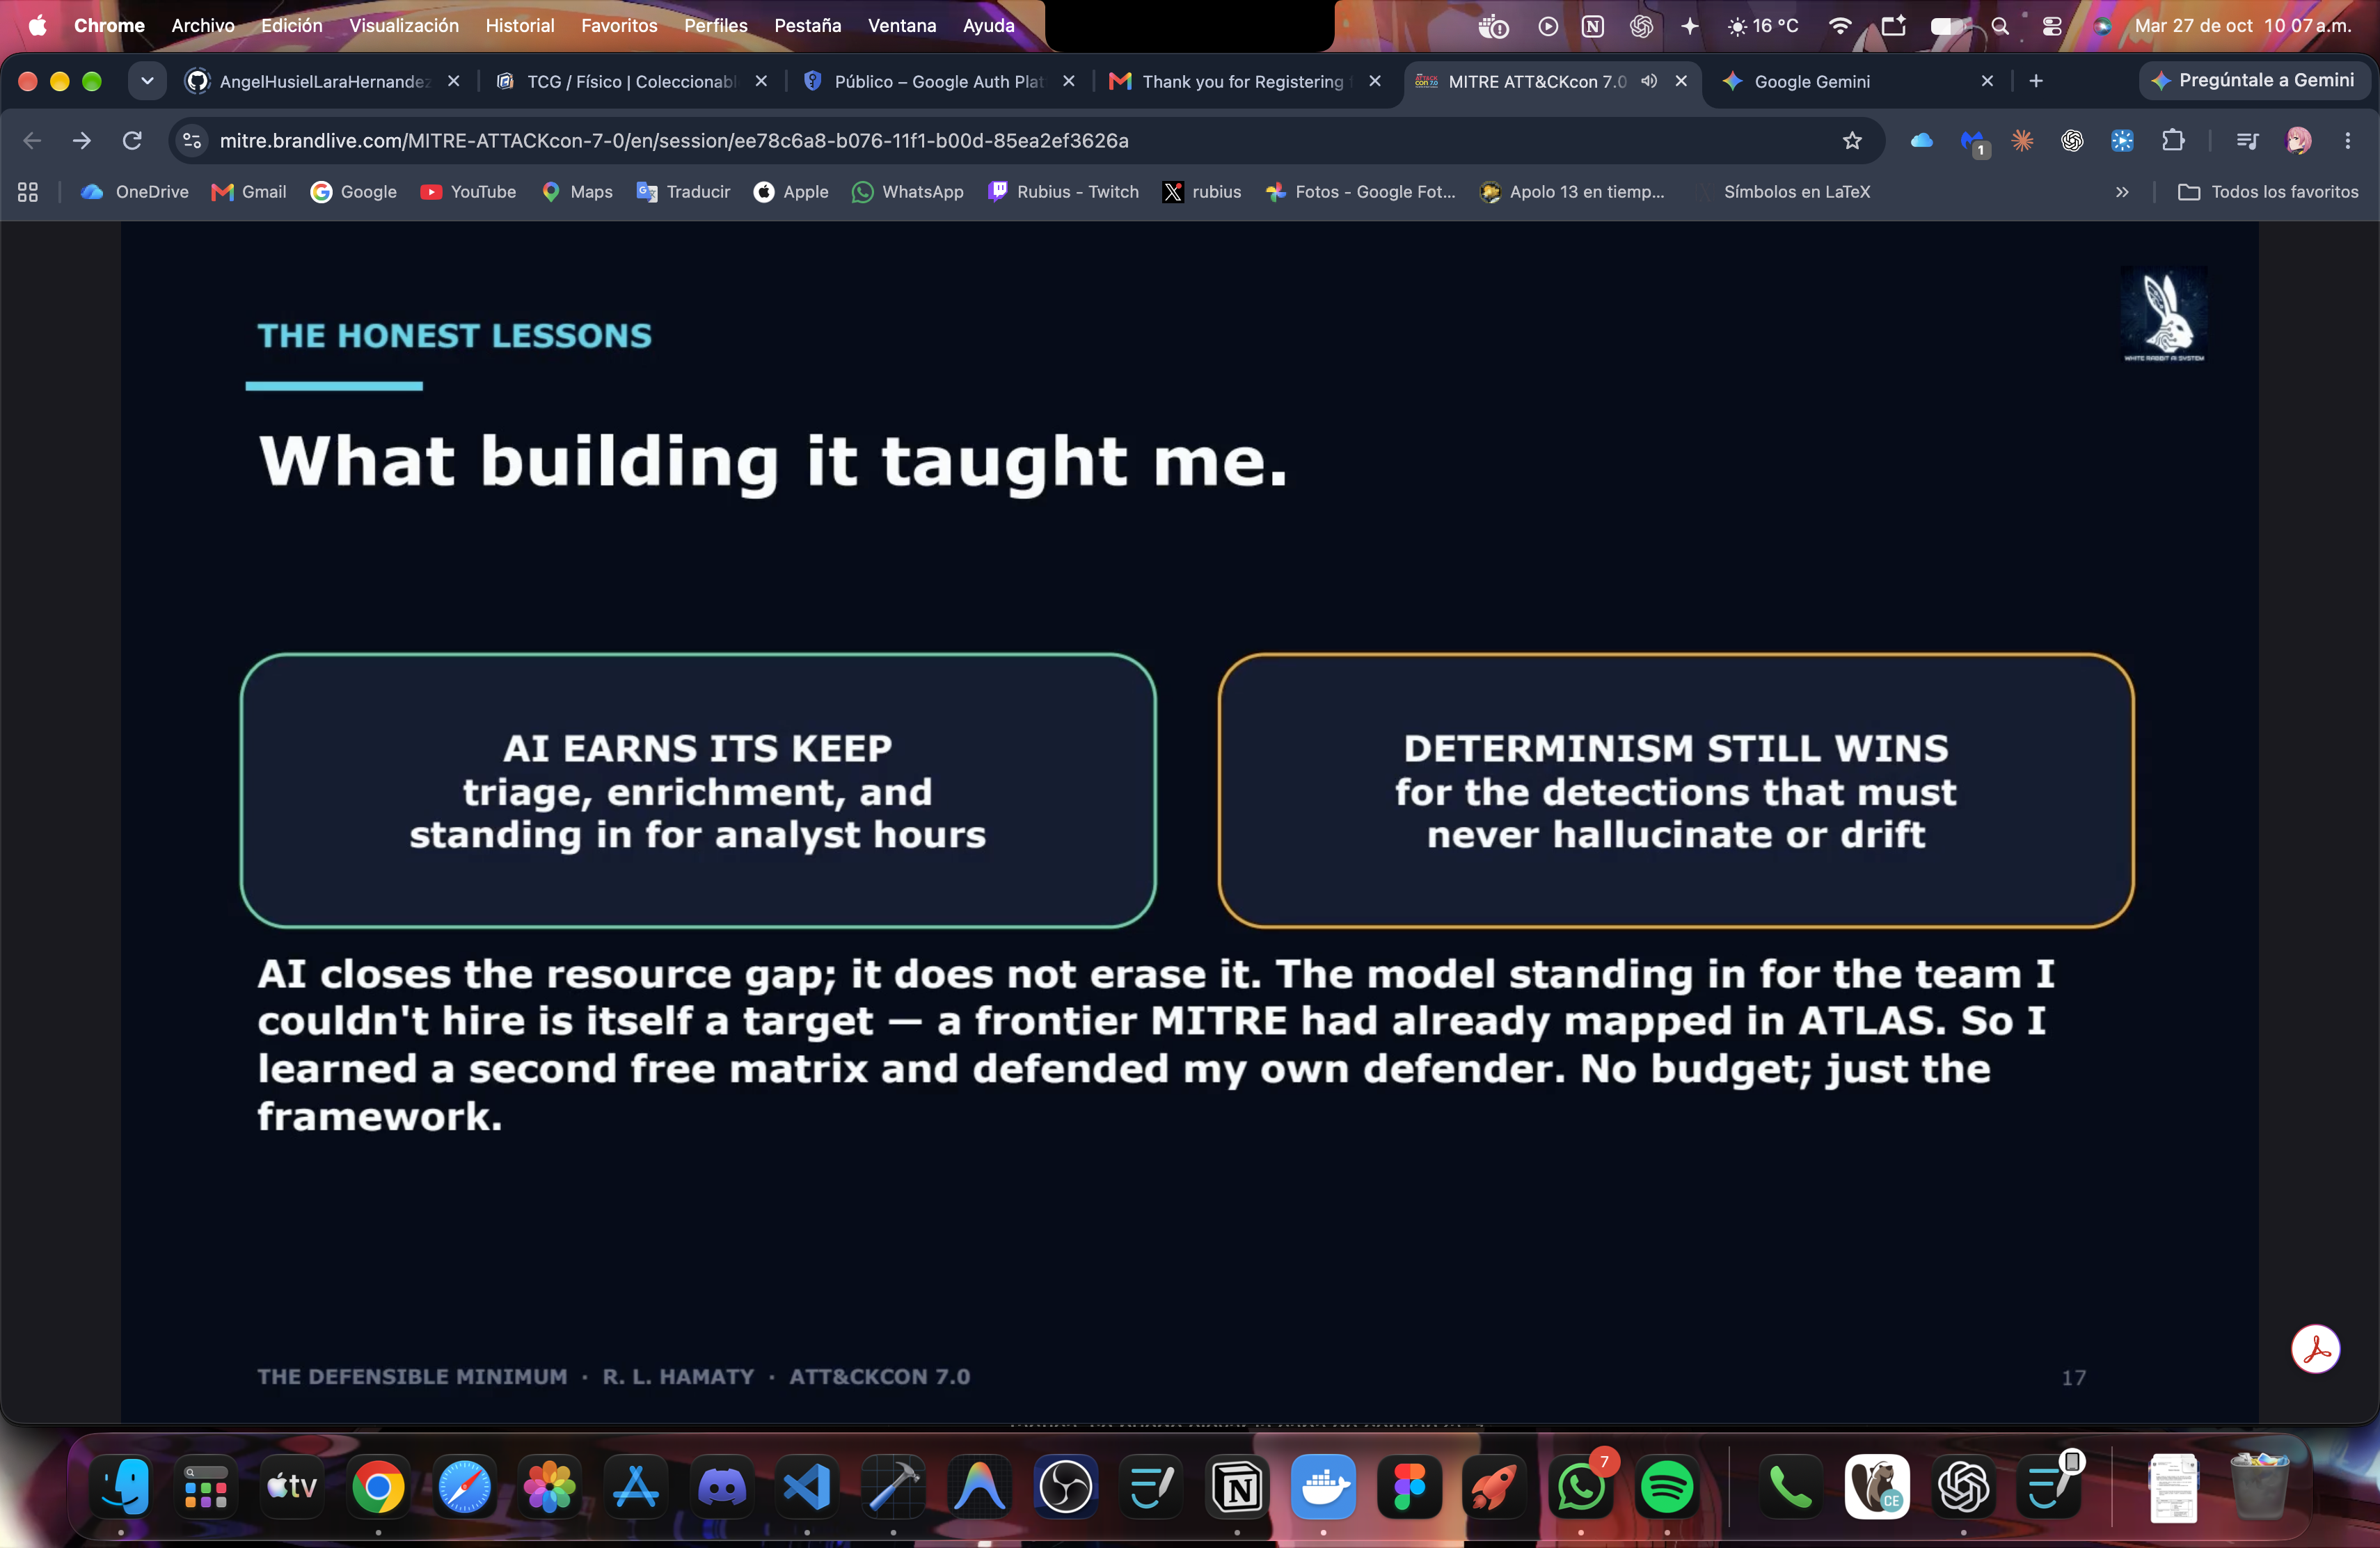
\includegraphics[width=1.0\textwidth]{img/image4.png}
    \caption{Uso de inteligencia artificial como apoyo y necesidad de detecciones comprobables.}
\end{figure}


Elementos a destacar:

\begin{itemize}
    \item Priorizar lo que es importante y se puede sostener con los recursos disponibles.
    \item Reconocer el riesgo que queda pendiente y validar de forma continua los controles.
\end{itemize}

\newpage
\subsection{MITRE ATT\&CK Updates: Enterprise ATT\&CK}

En esta charla se hablo de lo que se estaba preparando para la
version 21 de ATT\&CK, prevista para la primavera del 2027. Algo
que me llamo la atencion fue que el contenido relacionado con
inteligencia artificial, se
explico que primero era necesario revisar su alcance y la
evidencia del uso que le dan los adversarios.

\begin{figure}[H]
    \centering
    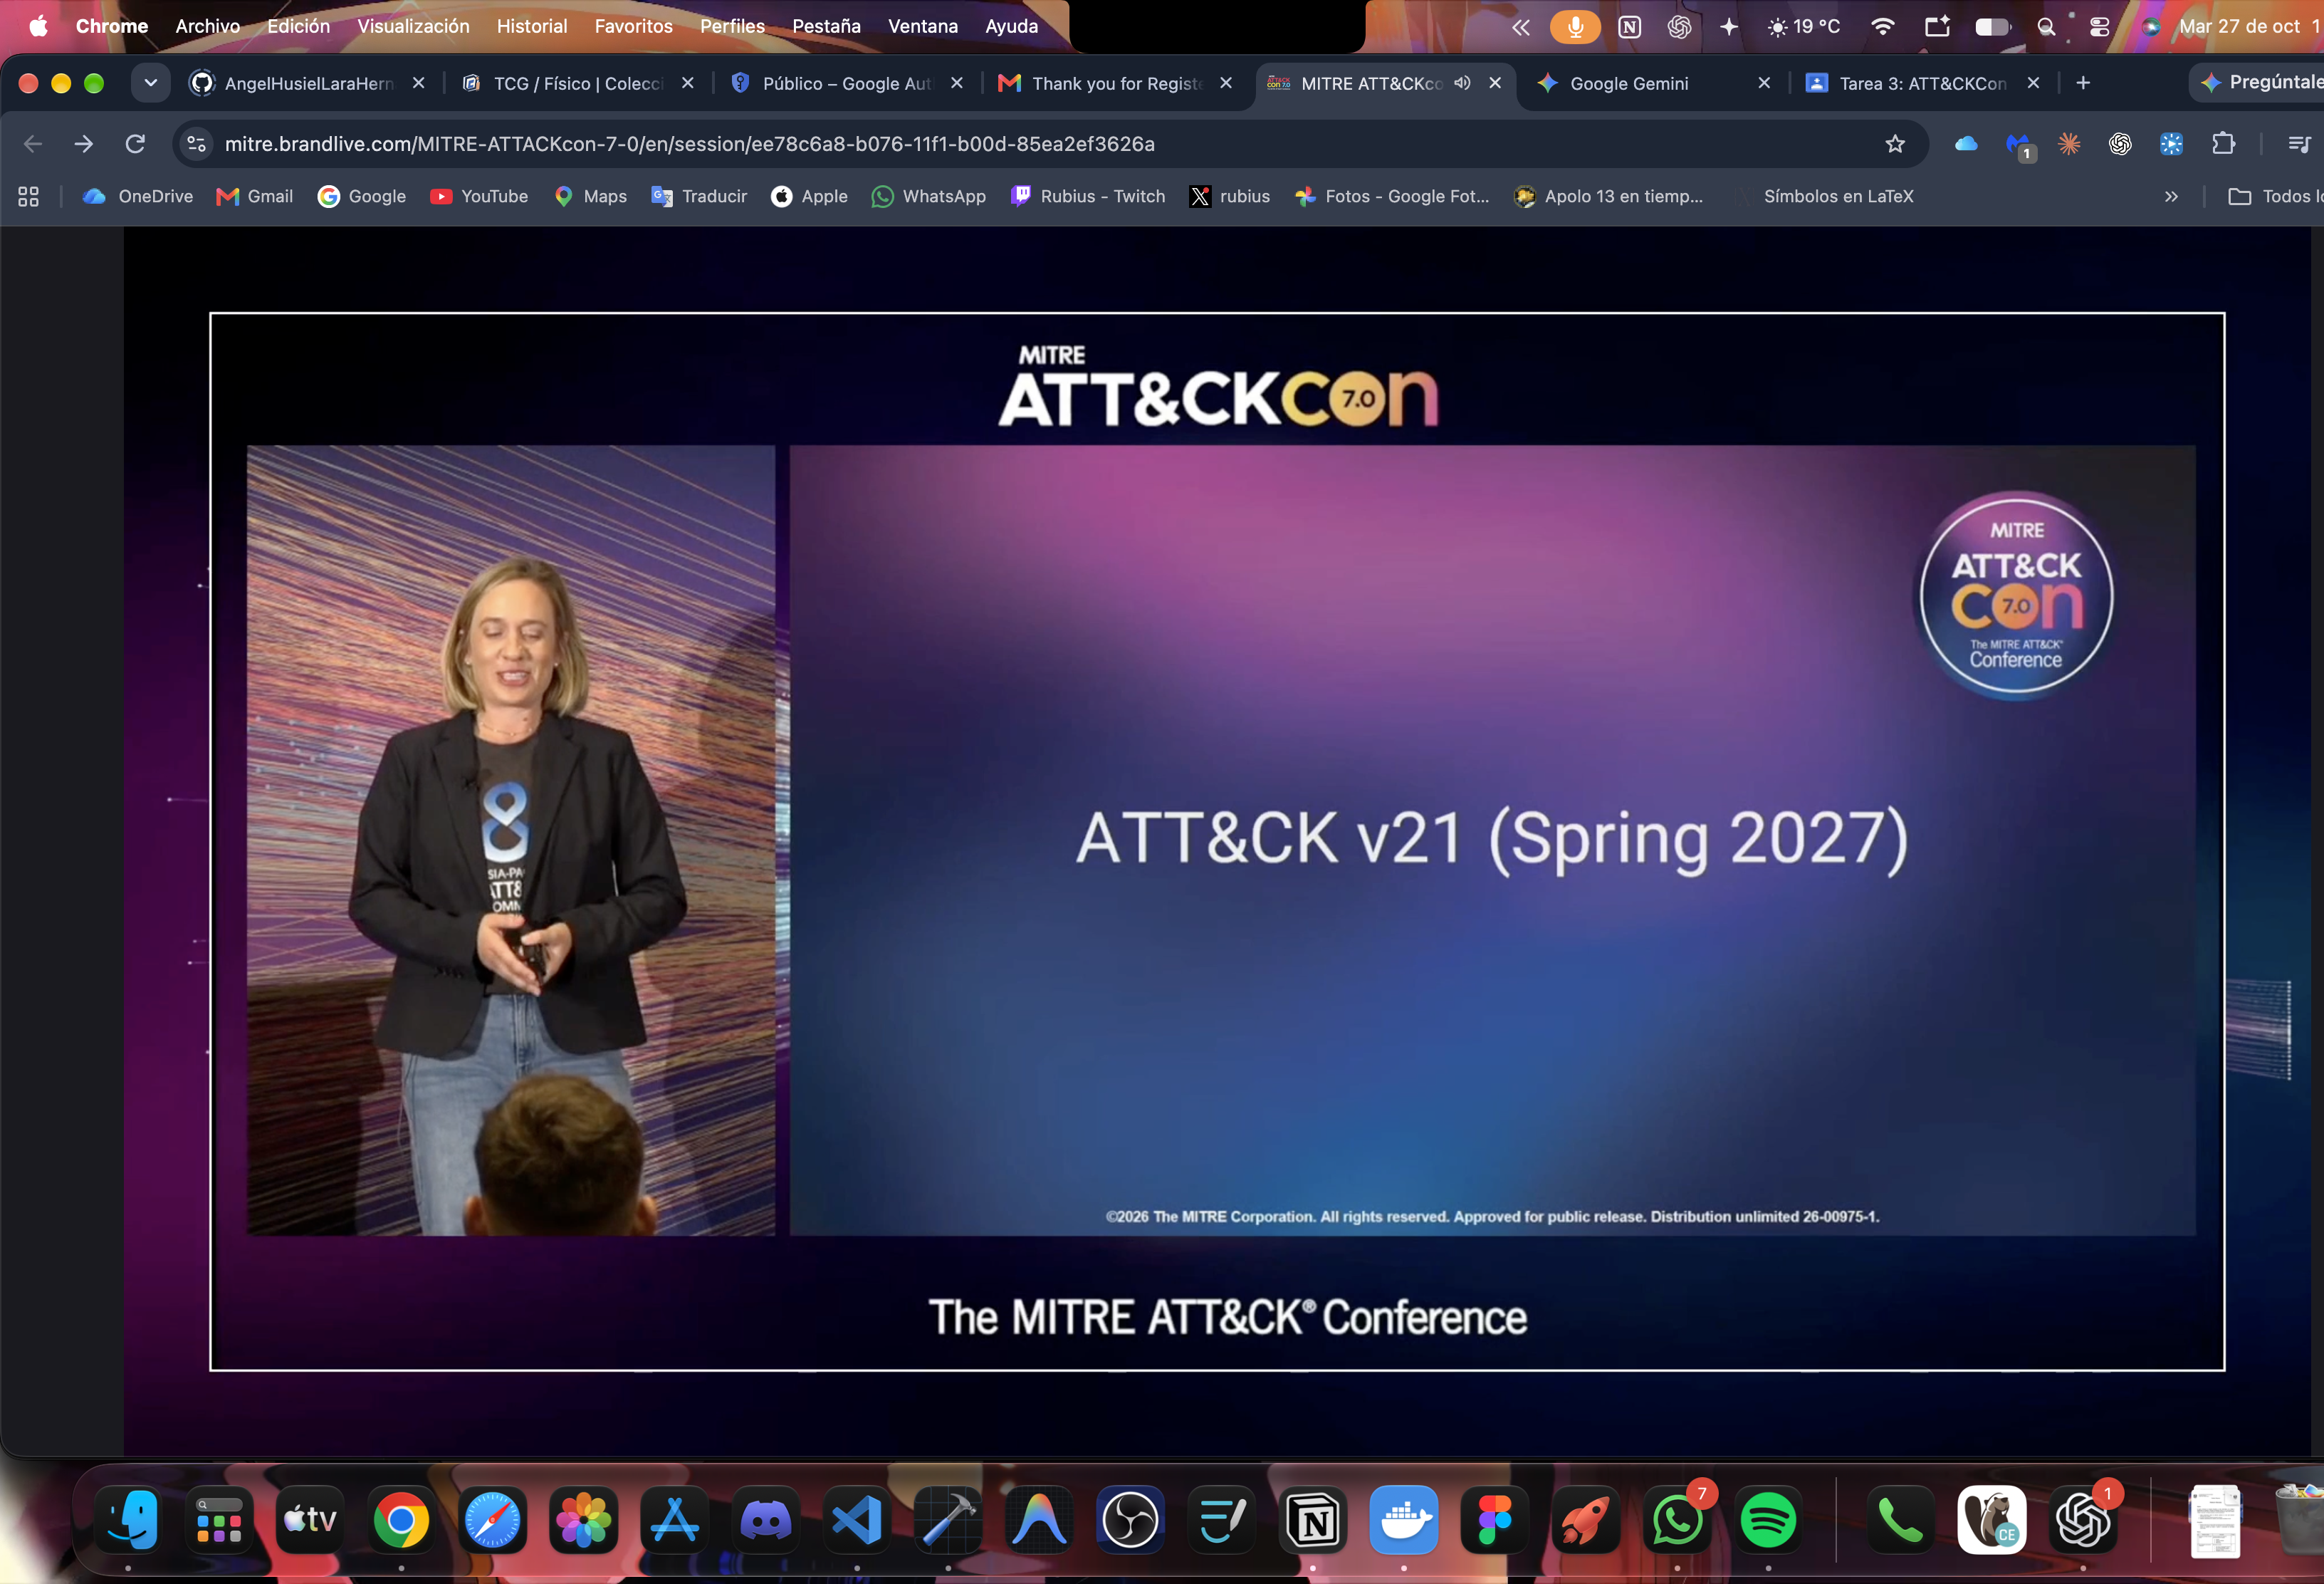
\includegraphics[width=1.0\textwidth]{img/image5.png}
    \caption{Presentacion de los planes para ATT\&CK v21 en la primavera del 2027.}
\end{figure}

Para esto, se hablo de MITRE ATLAS, que organiza conocimiento
sobre amenazas contra sistemas de inteligencia artificial. La
propuesta era que los equipos de ATLAS y ATT\&CK revisaran que
comportamientos podian incorporarse en Enterprise ATT\&CK. Donde
en este caso, se aclaro que las demostraciones o pruebas de
concepto no bastan por si solas para considerar que un
comportamiento ya tiene uso adversario real.

\begin{figure}[H]
    \centering
    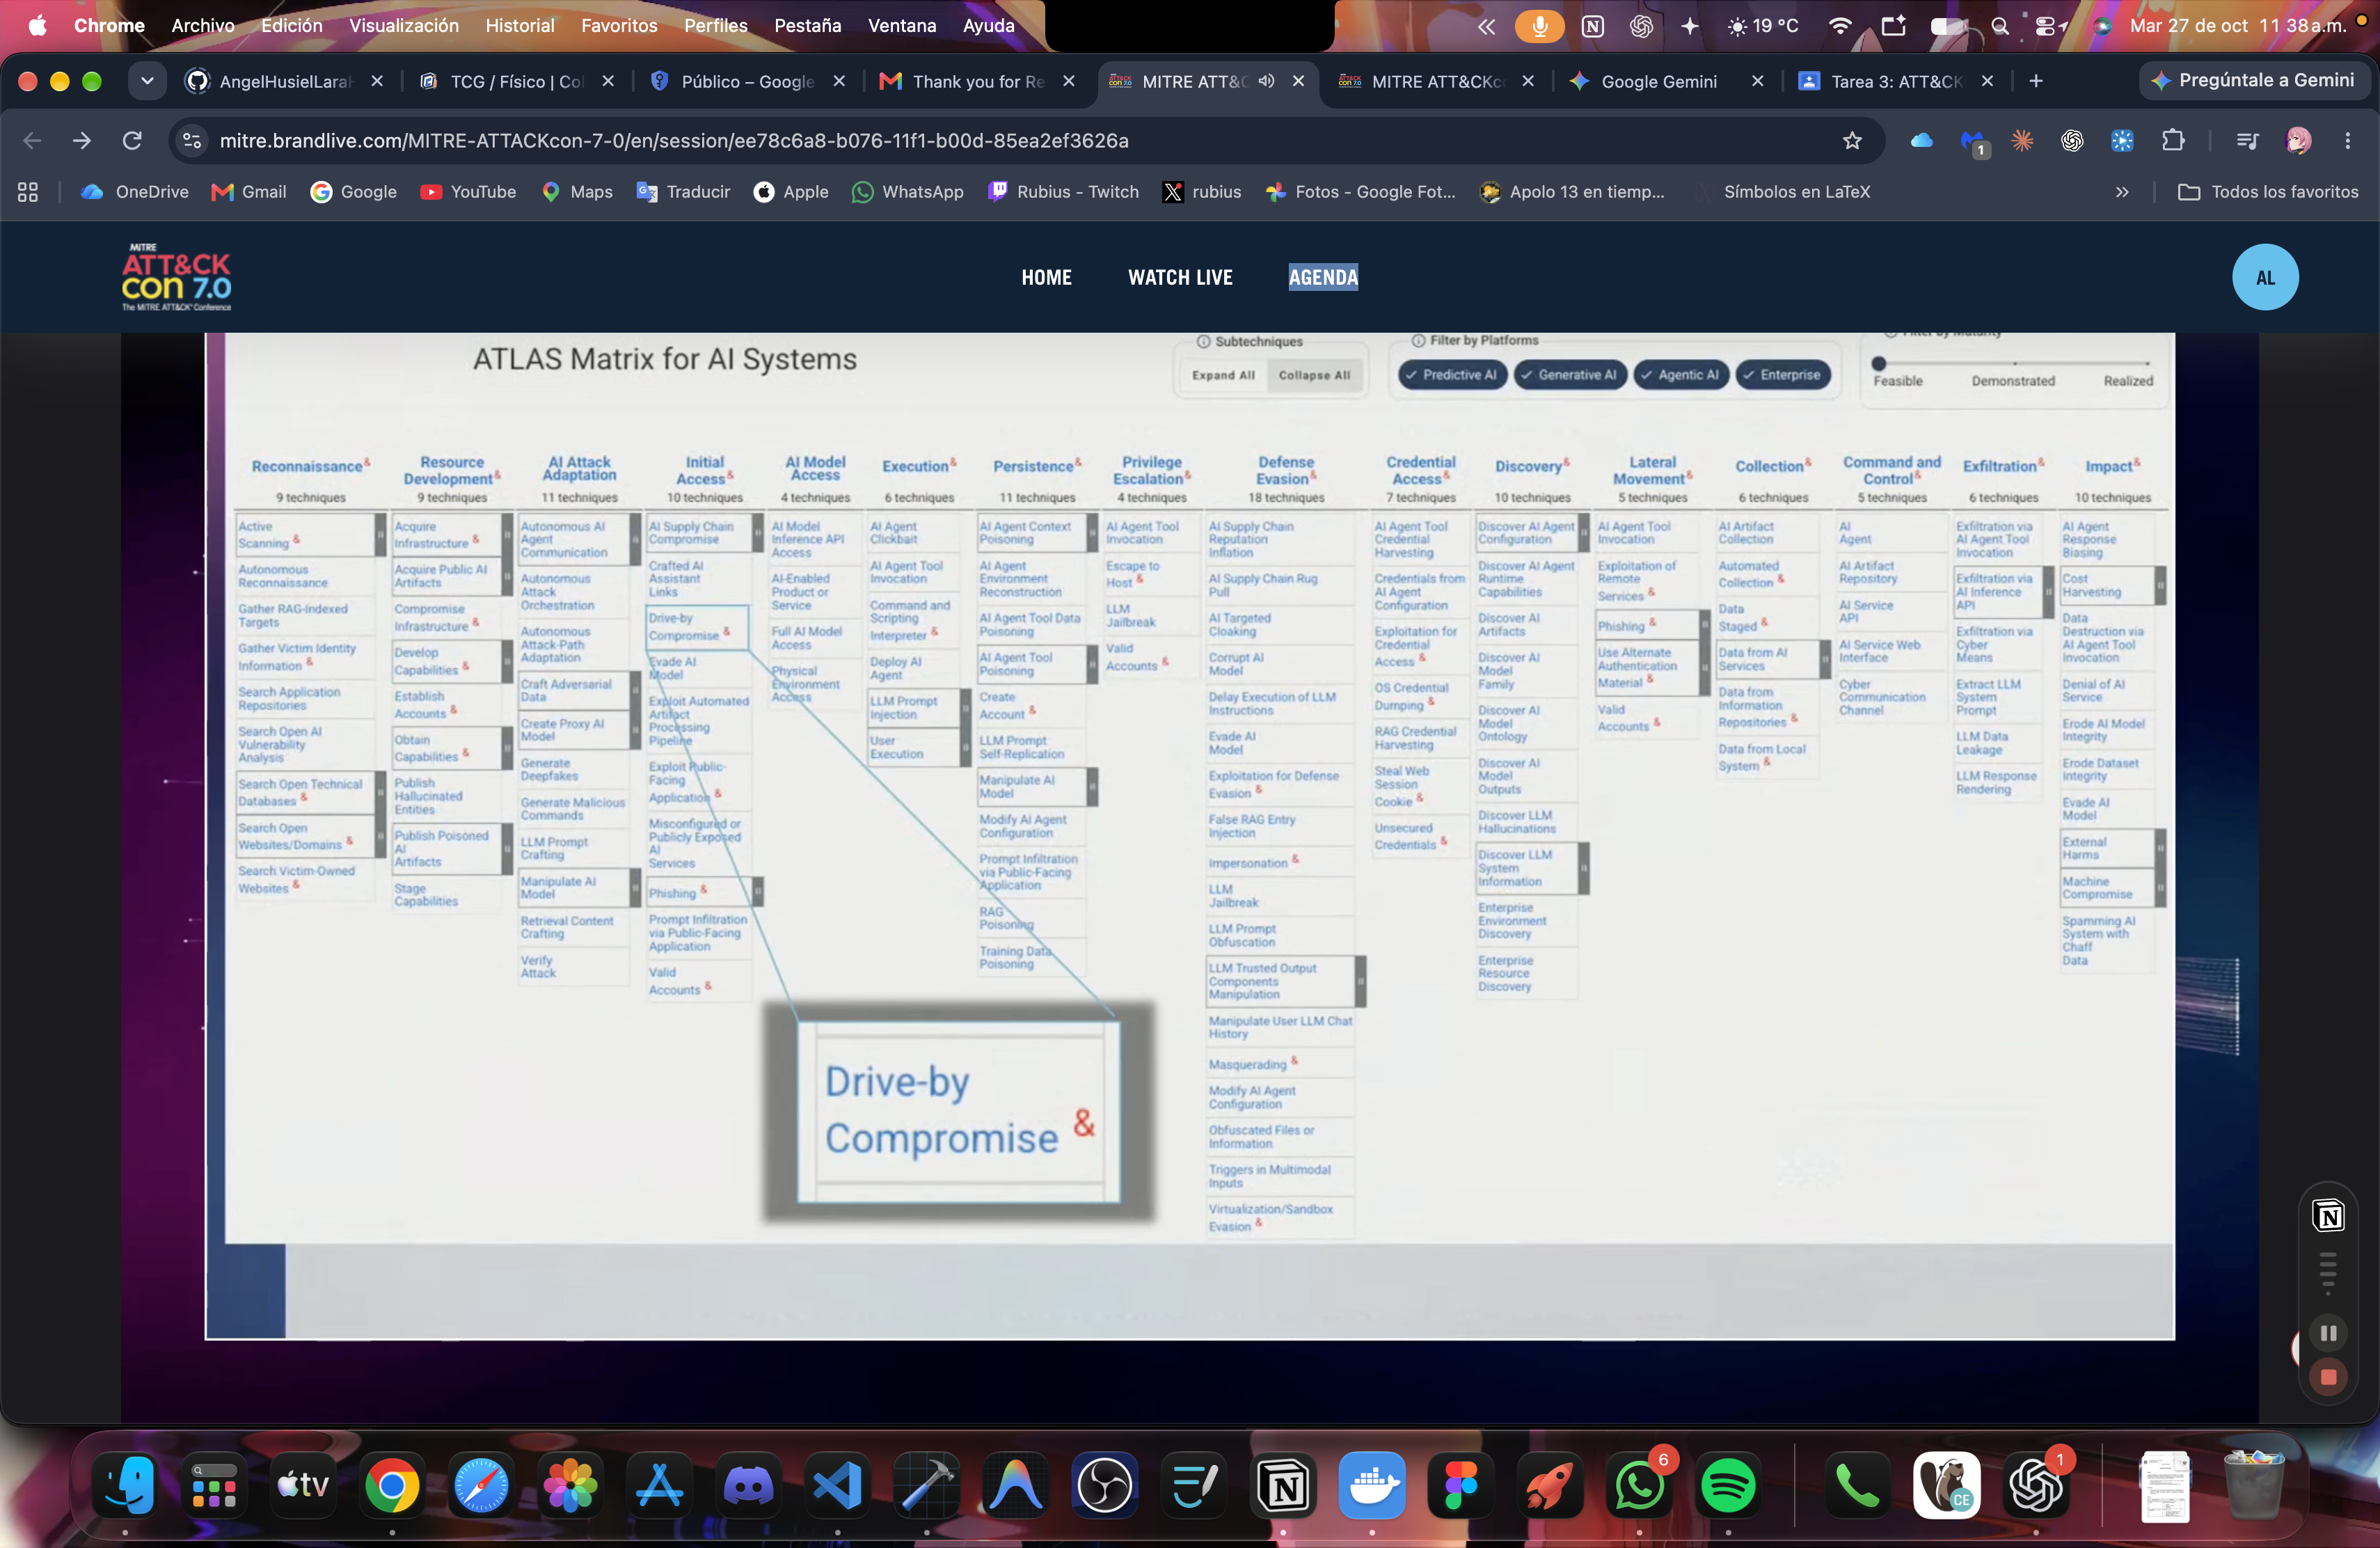
\includegraphics[width=0.5\textwidth]{img/image6.png}
    \caption{Matriz de ATLAS utilizada para explicar la relacion con Enterprise ATT\&CK.}
\end{figure}

Despues de esto se explicaron varias posibilidades. Parte del
contenido podria añadirse a una tecnica que ya existe, otra parte
podria necesitar una nueva subtecnica o una tecnica especifica, y
algunos comportamientos podrian permanecer fuera mientras no
cumplan los criterios.

Un ejemplo fue el AI Artifact Repository, donde un repositorio de
artefactos de IA puede utilizarse como un canal para intercambiar
instrucciones o resultados dentro de una operacion.

\begin{figure}[H]
    \centering
    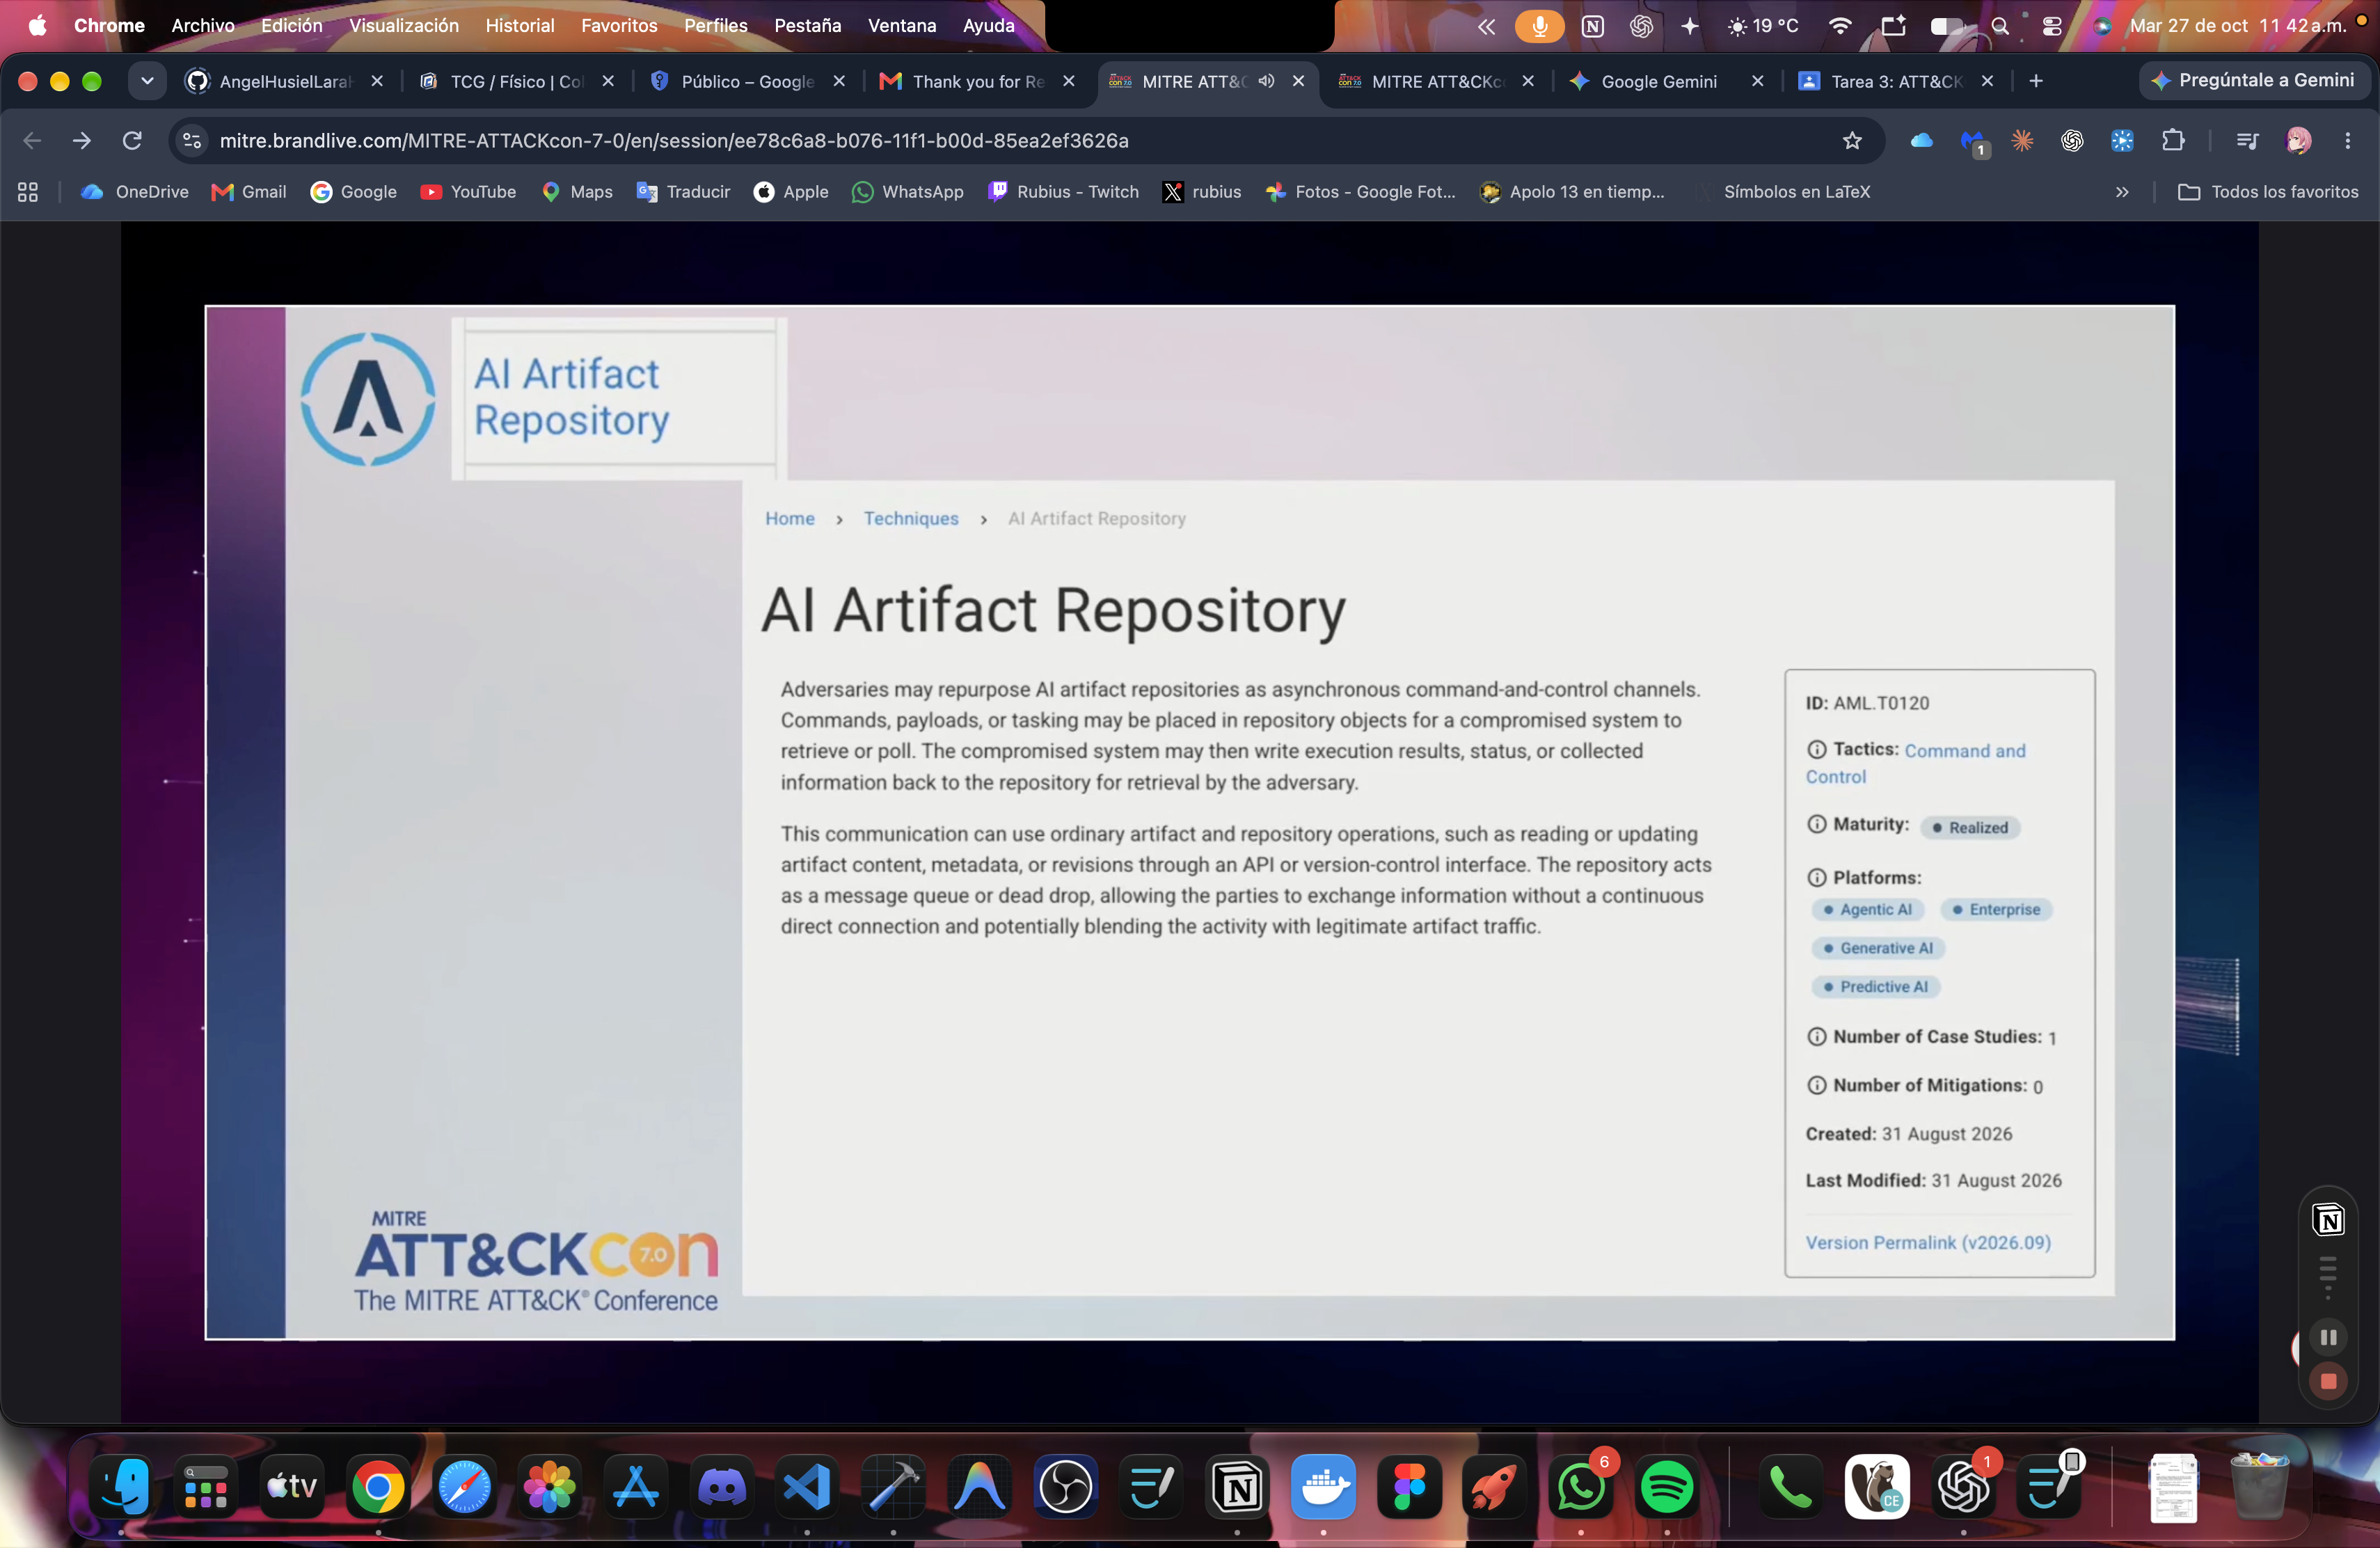
\includegraphics[width=0.5\textwidth]{img/image10.png}
    \caption{Ejemplo de uso de un repositorio de artefactos de IA como canal de comunicacion.}
\end{figure}

Elementos a destacar:

\begin{itemize}
    \item Revisar el uso adversario real antes de incorporar un comportamiento.
    \item Distinguir lo que se puede integrar en una tecnica existente de lo que necesita otra clasificacion.
    \item Considerar las conexiones del sistema de IA con otros recursos de la organizacion.
\end{itemize}

\newpage
\subsection{Measuring ATT\&CK Coverage Through Real Malware Tradecraft}

El ejemplo principal fue T1055, Process Injection,
que se refiere a ejecutar codigo dentro del espacio de otro
proceso. La idea que mas me llamo la atencion fue que decir que
detectar este ataque puede significar cosas muy distintas,
dependiendo de que procedimiento se probo y de que datos se
recolectaron.

Para esto se separaron varios niveles: la tecnica que se quiere
estudiar, el procedimiento con el que un programa la implementa,
el comportamiento que se puede observar y la capacidad de
deteccion del sensor. Donde en este caso, que un procedimiento
exista no significa que nuestro equipo vaya a generar toda la
informacion necesaria para reconocerlo.

Despues se comparo con T1059, relacionado con interpretes de
comandos y scripts. En ese caso, una linea de comandos puede
aportar evidencia importante sobre la ejecucion. No obstante,
para varias formas de inyeccion es necesario revisar accesos
entre procesos, cambios en la memoria, permisos o cargas de
componentes. 

Si se prueban
ocho procedimientos y solamente se pueden validar cinco, eso
representa el 62.5\% de esos ocho procedimientos. No significa
que se pueda detectar el 62.5\% de todos los ataques que existen.


Elementos destacods 

\begin{itemize}
    \item Distinguir entre tecnica, procedimiento, evidencia observable y deteccion.
    \item Medir la cobertura sobre los procedimientos que realmente se probaron.
    \item Volver a validar las detecciones cuando cambian las implementaciones o el entorno.
\end{itemize}

\Needspace{10\baselineskip}
\subsection{Breaking the Defenders}

Ahora bien, la idea principal fue distinguir entre ocultar una
accion y afectar la capacidad de las defensas. Se puede detener
un servicio de seguridad, pero tambien se puede alterar lo que
observa sin que el proceso desaparezca. Por lo que, ver un
servicio en ejecucion no demuestra que siga entregando
informacion util.

Para esto, se mencionaron ejemplos de interferencia con
mecanismos de Windows que ayudan a revisar scripts o generar
eventos, como AMSI y ETW. Tambien se hablo del abuso de
controladores vulnerables y de cambios en la carga de librerias.

De igual forma, se revisaron casos de ransomware, donde borrar
respaldos o impedir la recuperacion puede cambiar las
posibilidades de respuesta de una organizacion. No obstante, se
explico que no basta con esperar hasta el cifrado o hasta que
aparezca la nota de rescate, por que para ese momento ya se
perdieron varias oportunidades de detectar la preparacion del
ataque.

\begin{figure}[H]
    \centering
    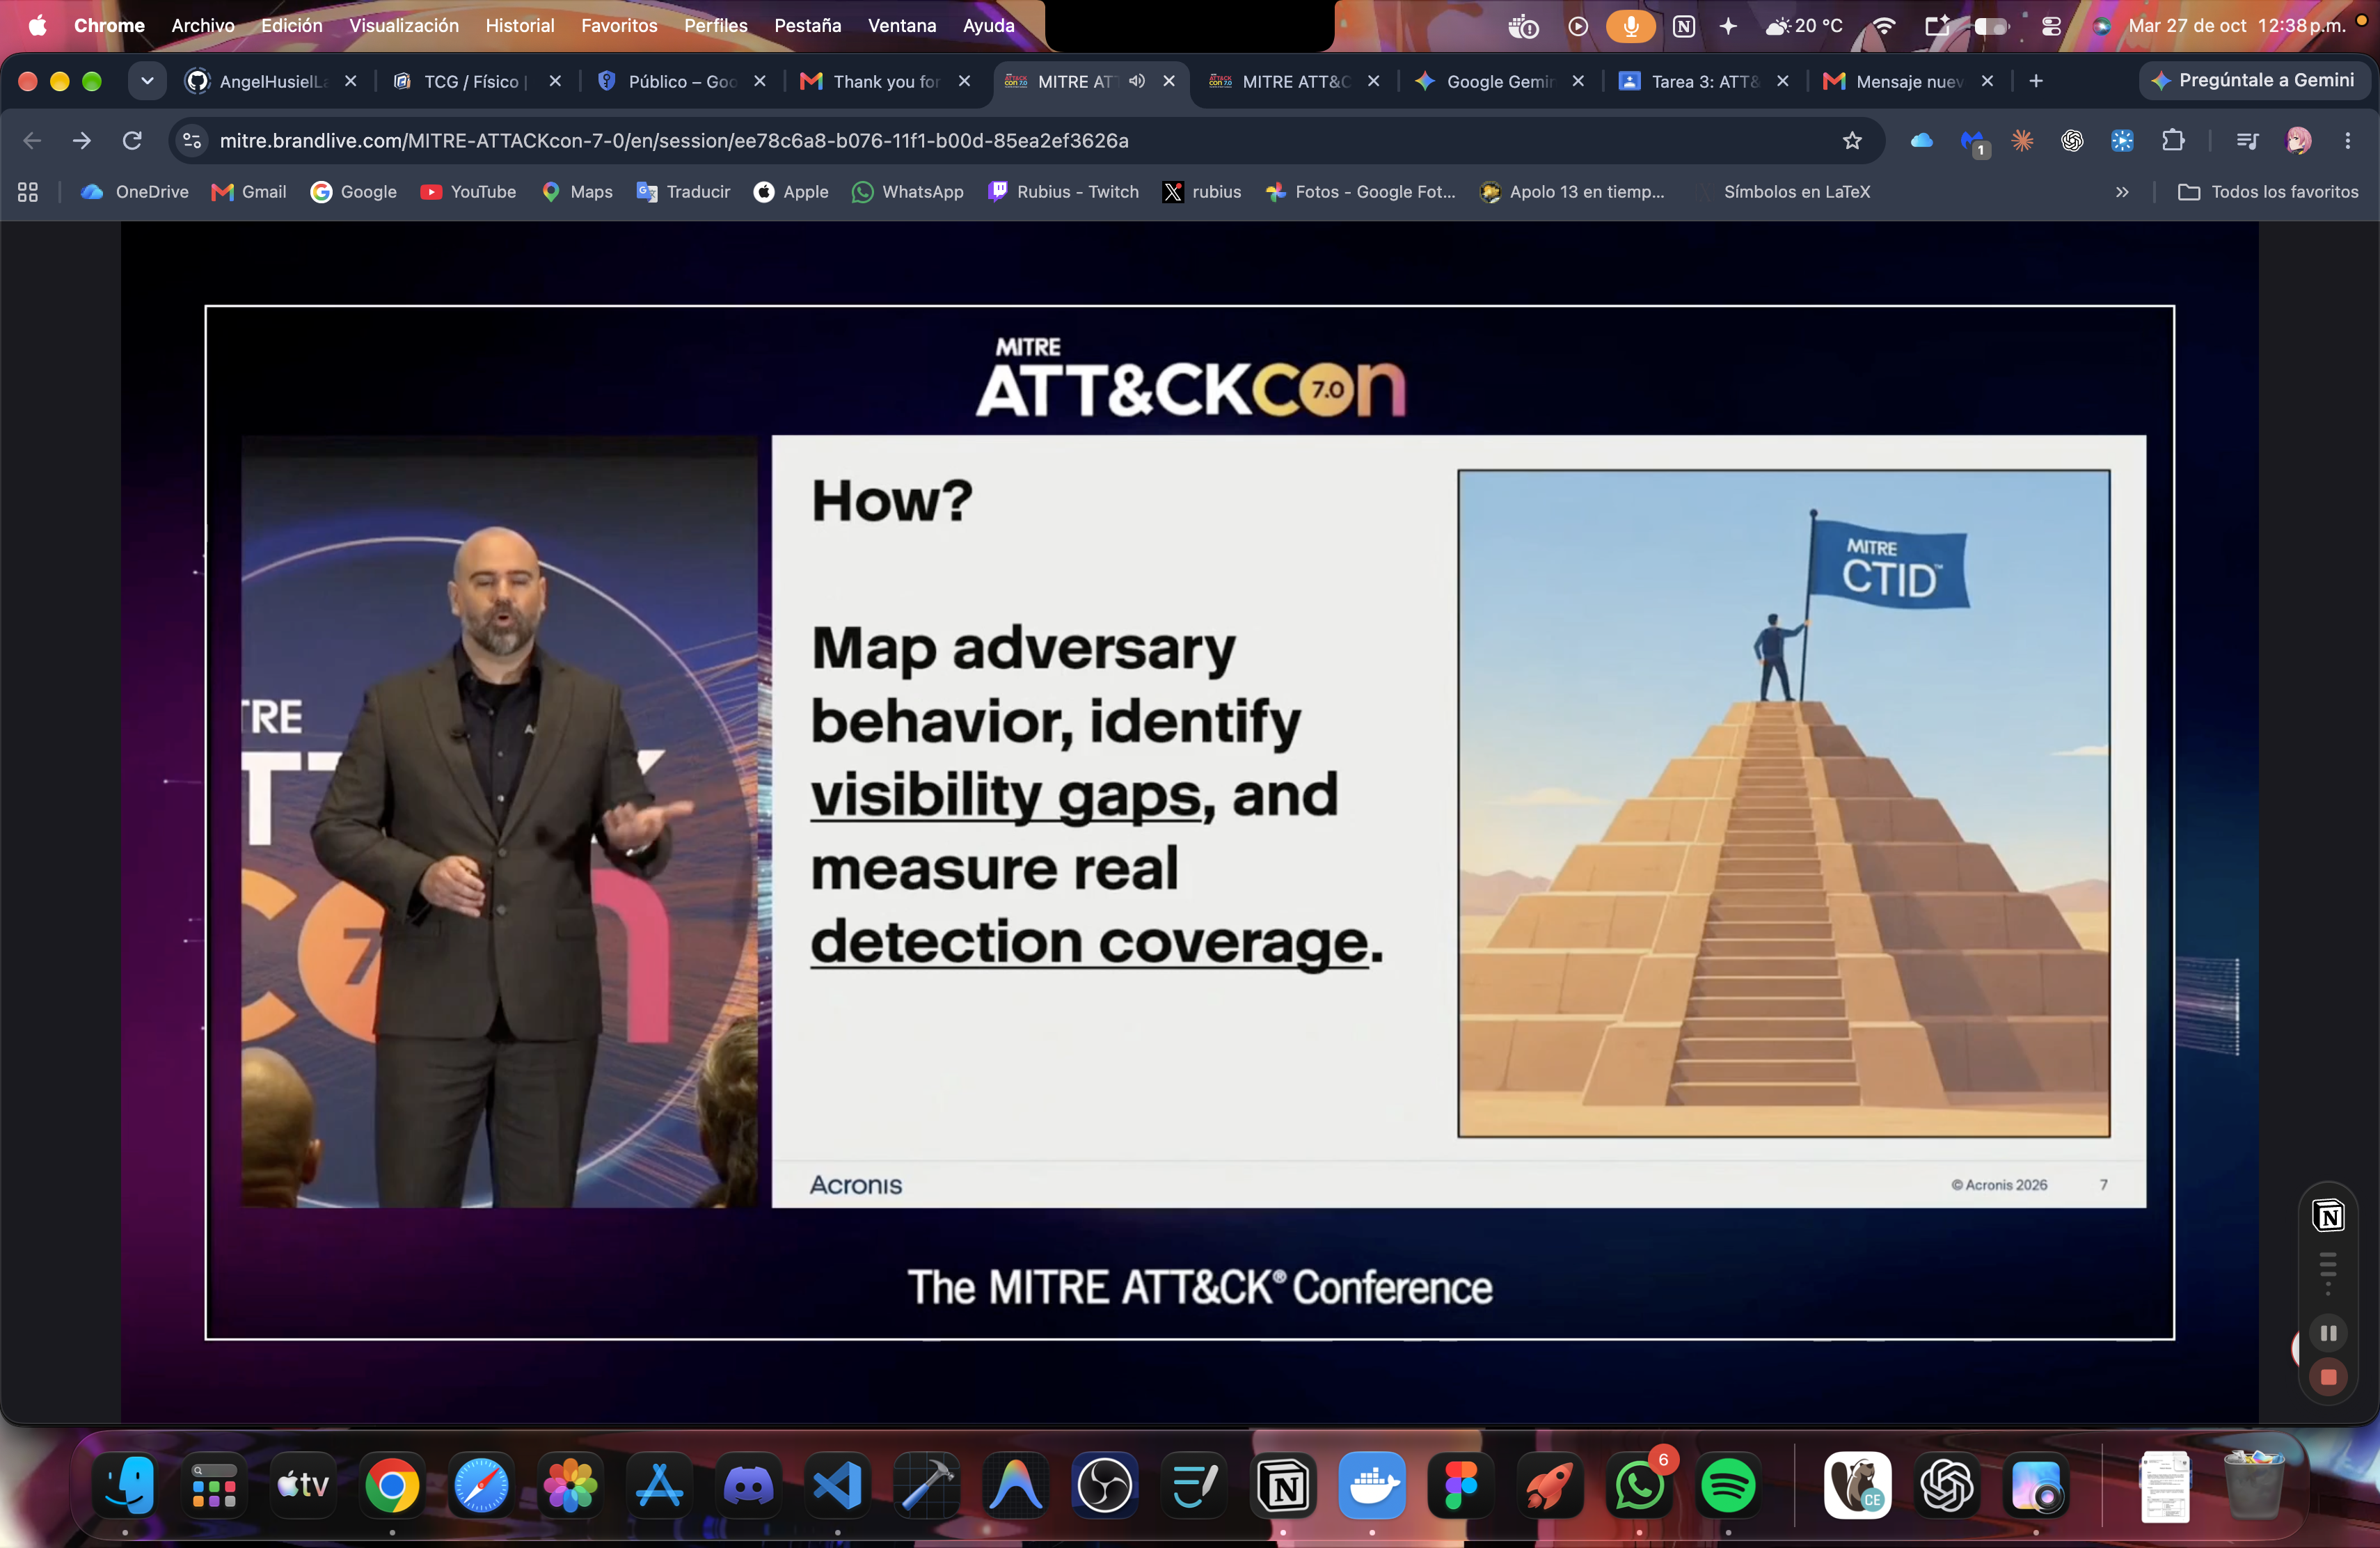
\includegraphics[width=0.5\textwidth]{img/image13.png}
    \caption{Mapeo del comportamiento, identificacion de falta de visibilidad y medicion de la cobertura real.}
\end{figure}


Por ultimo, se hablo de los MSP, que son proveedores que
administran servicios para distintos clientes. Una configuracion
que funciona para uno puede generar mucho ruido para otro, por lo
que cada entorno necesita sus propios criterios. Con esto me
quedo con que la cobertura tambien depende de comprobar que el
defensor sigue pudiendo ver, no solamente de tener una lista de
reglas configuradas.

Los elementos a destacar fueron:

\begin{itemize}
    \item Revisar tanto los intentos de afectar una defensa como sus consecuencias.
    \item Investigar la perdida de telemetria con otras fuentes y con el contexto del equipo.
    \item Adaptar las detecciones a cada cliente y comprobar que los sensores siguen siendo utiles.
\end{itemize}

\newpage
\section{Ejemplos del uso de ATT\&CK en la industria}

\begin{enumerate}
    \item \textbf{Ingenieria de deteccion en un SOC.} Relacionar una tecnica con los registros que se necesitan, revisar la cadena de procesos y comprobar si el SIEM genera una alerta con un caso de prueba. El SOC es el equipo que revisa y responde a este tipo de eventos.
    \item \textbf{Investigacion de identidades en servicios SaaS.} Conectar accesos, cambios en cuentas y acciones dentro de las aplicaciones, para revisar la progresion de una posible intrusion y no solamente eventos aislados.
    \item \textbf{Defensa de organizaciones con pocos recursos.} Priorizar las amenazas mas relevantes y los controles que se pueden mantener, dejando claro que riesgos siguen pendientes.
    \item \textbf{Validacion de productos y sensores.} Probar varios procedimientos de una tecnica y revisar que evidencia se obtiene, antes de afirmar que existe cobertura.
    \item \textbf{Monitoreo de las propias defensas.} Relacionar la perdida de registros con otros eventos para investigar si un control dejo de funcionar o fue afectado.
    \item \textbf{Proteccion de sistemas de IA.} Utilizar el conocimiento de ATLAS y revisar su relacion con ATT\&CK, considerando tambien las integraciones que conectan esos sistemas con otros recursos.
\end{enumerate}



\section{Experiencia general y relacion con la materia}

En la practica 5 se obtuvieron credenciales, en la 6 se revisaron el
sistema y la red interna, y en la 7 se utilizo un tunel SSH para
acceder a otro equipo. Ahora bien, durante el evento pude ver
como esas acciones tambien se pueden estudiar desde lo que
tendria que observar un defensor.

Del otro lado se tendria
que revisar si se registro el acceso, si se reconocio la cuenta,
si aparecieron conexiones nuevas y si alguien relaciono esos
datos. Esta relacion me ayudo a pensar en que registros serian
necesarios para reconocer los procedimientos que realizamos
durante las practicas.

Otro elemento que me llamo la atencion dentro del evento fue un
ejemplo de MalChela conectado con Claude por medio de MCP. Se
mostro una integracion para que una interfaz de IA pudiera
utilizar herramientas del proyecto. Esto se relaciona con las
preguntas sobre las conexiones de la IA con otros recursos: entre
mas herramientas puede utilizar, mas importante se vuelve
entender a que puede acceder y que acciones se le permiten.

\begin{figure}[H]
    \centering
    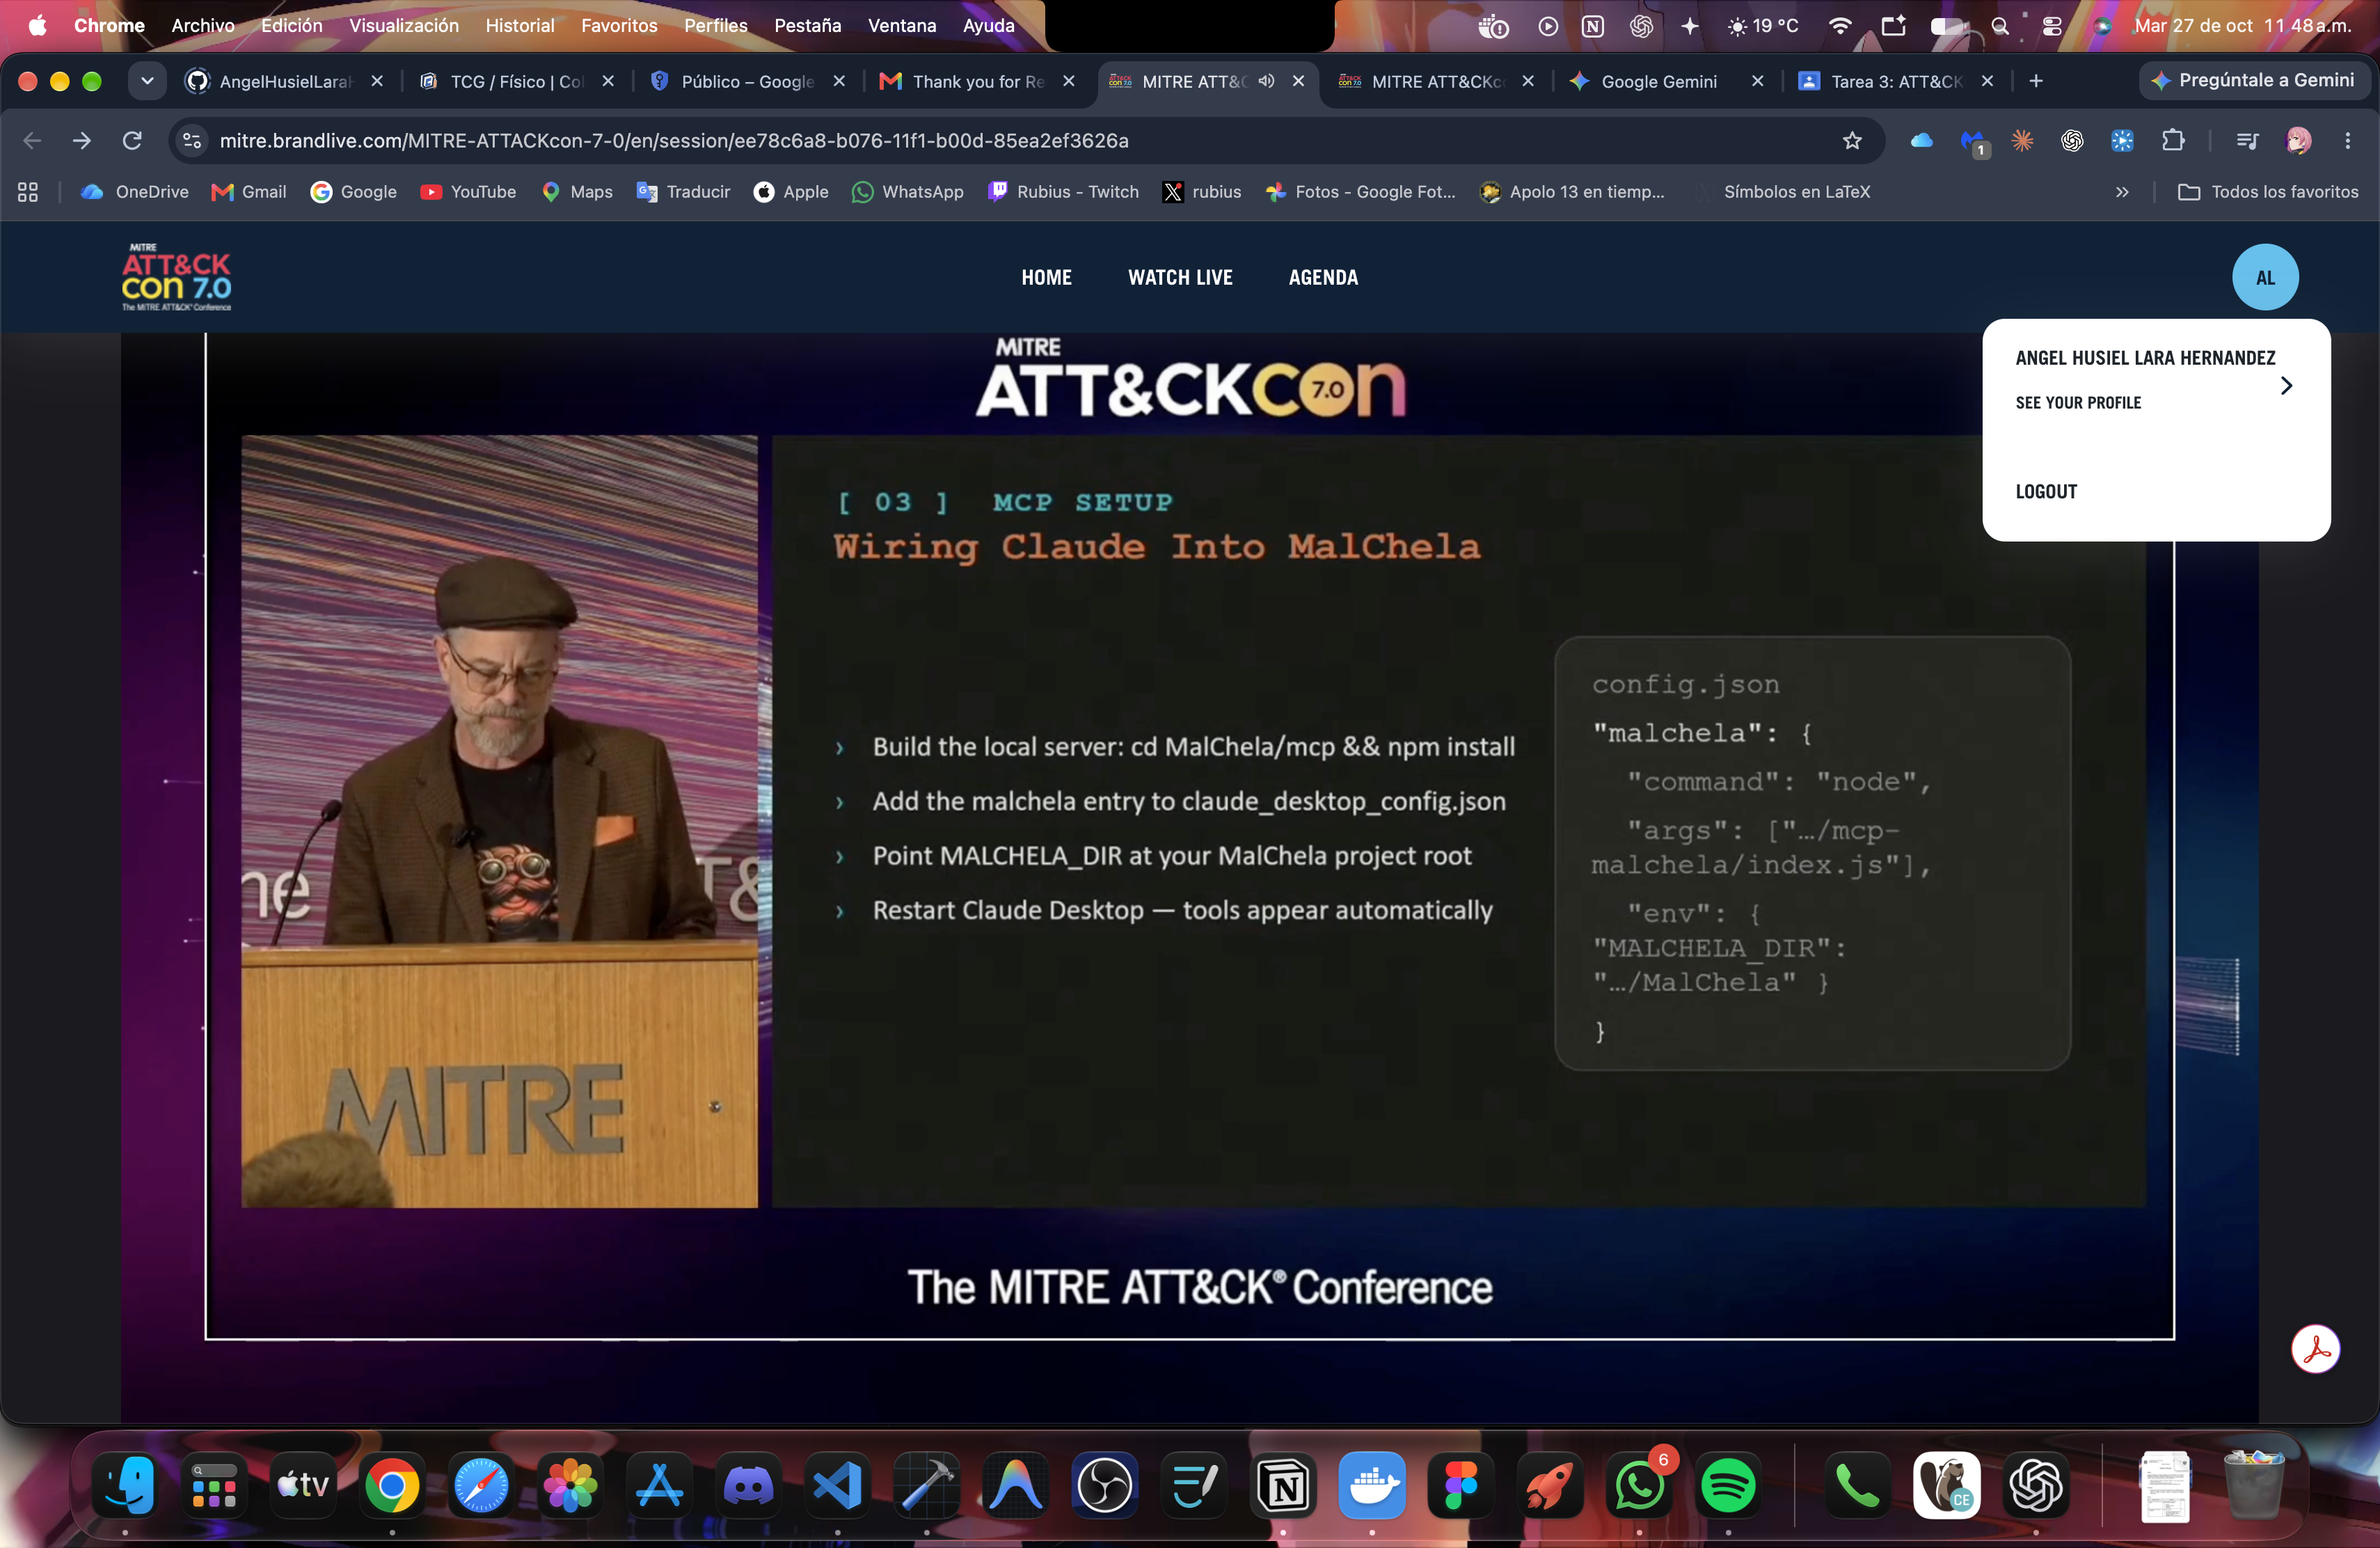
\includegraphics[width=\textwidth,trim=130.01bp 92.00bp 100.01bp 235.01bp,clip]{img/image11.png}
    \caption{Ejemplo de integracion de Claude con herramientas de MalChela mediante MCP.}
\end{figure}


Por ultimo, me parecio importante que varias presentaciones
señalaran lo que todavia no estaba resuelto: el alcance de una
futura plataforma de IA, los procedimientos que no se habian
validado o las amenazas que una organizacion no puede cubrir
todavia. Esto me hizo sentido por que reconocer esos limites
permite saber que falta por mejorar, en lugar de asumir que todo
esta completo.

\section{Evidencia de participacion en el evento}

Para participar me registre en la modalidad virtual de ATT\&CKcon
7.0 y recibi el correo de confirmacion. 

\begin{figure}[H]
    \centering
    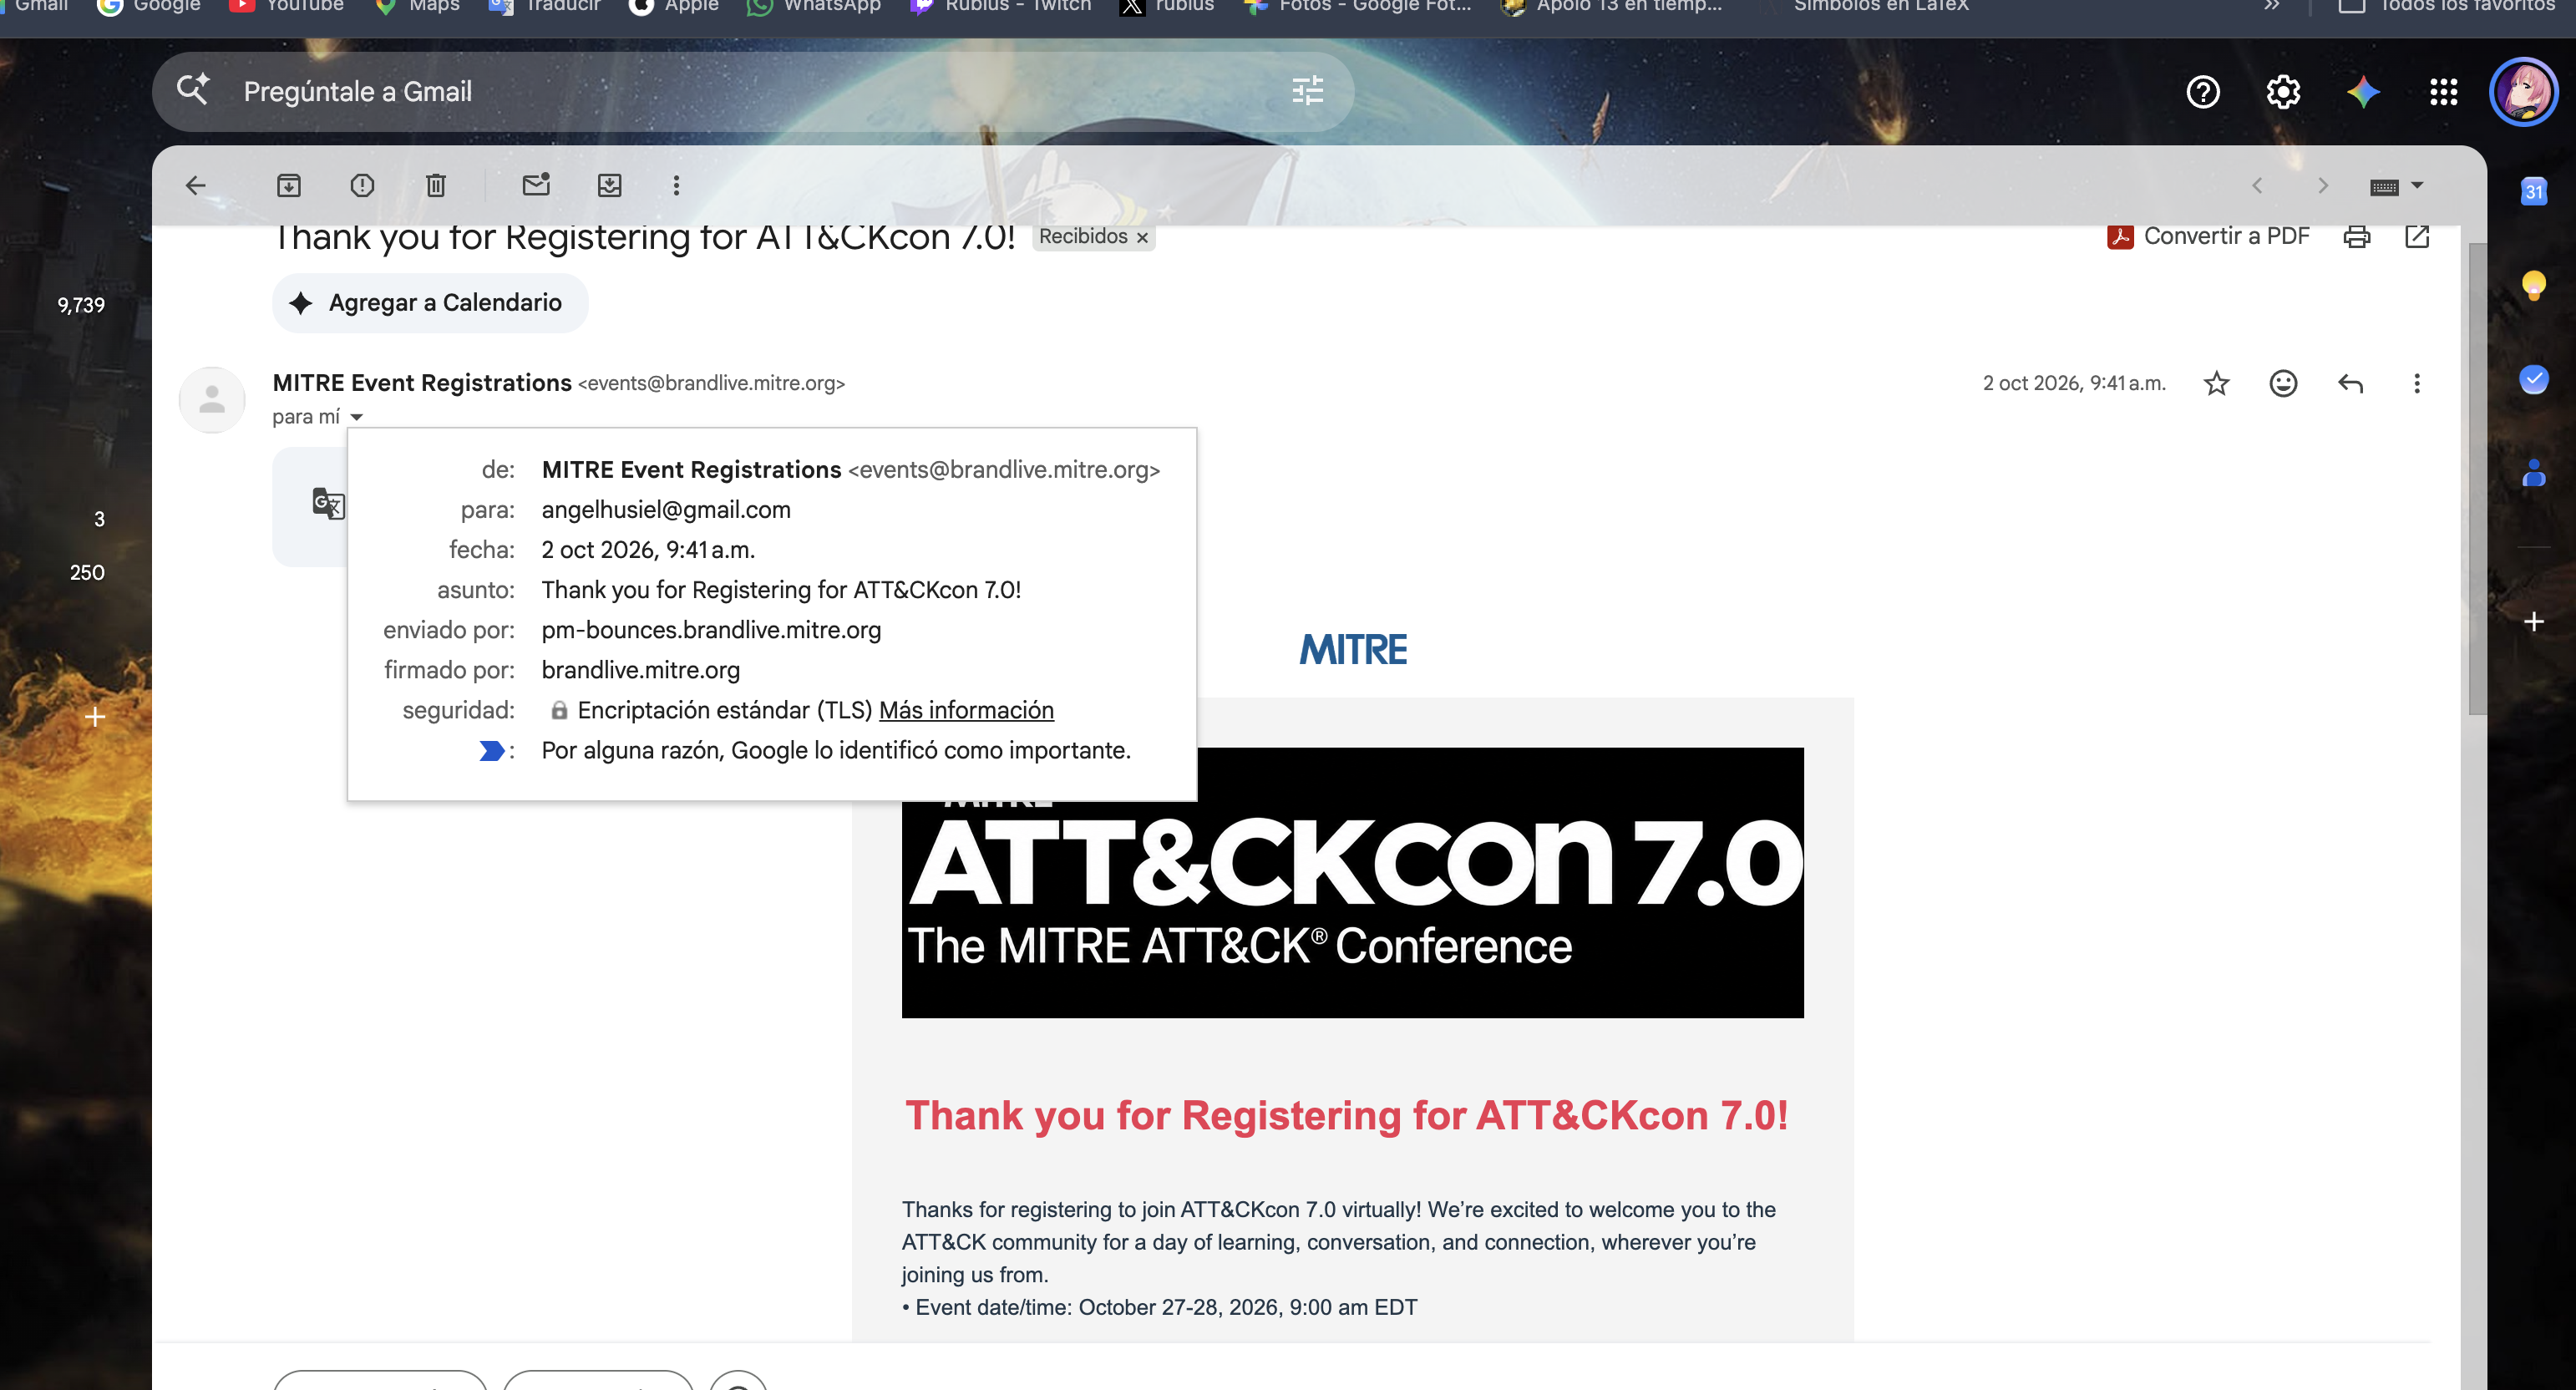
\includegraphics[width=0.95\textwidth,trim=100.01bp 12.00bp 52.00bp 135.01bp,clip]{img/image1.png}
    \caption{Confirmacion del registro a ATT\&CKcon 7.0 en modalidad virtual.}
\end{figure}

\begin{figure}[H]
    \centering
    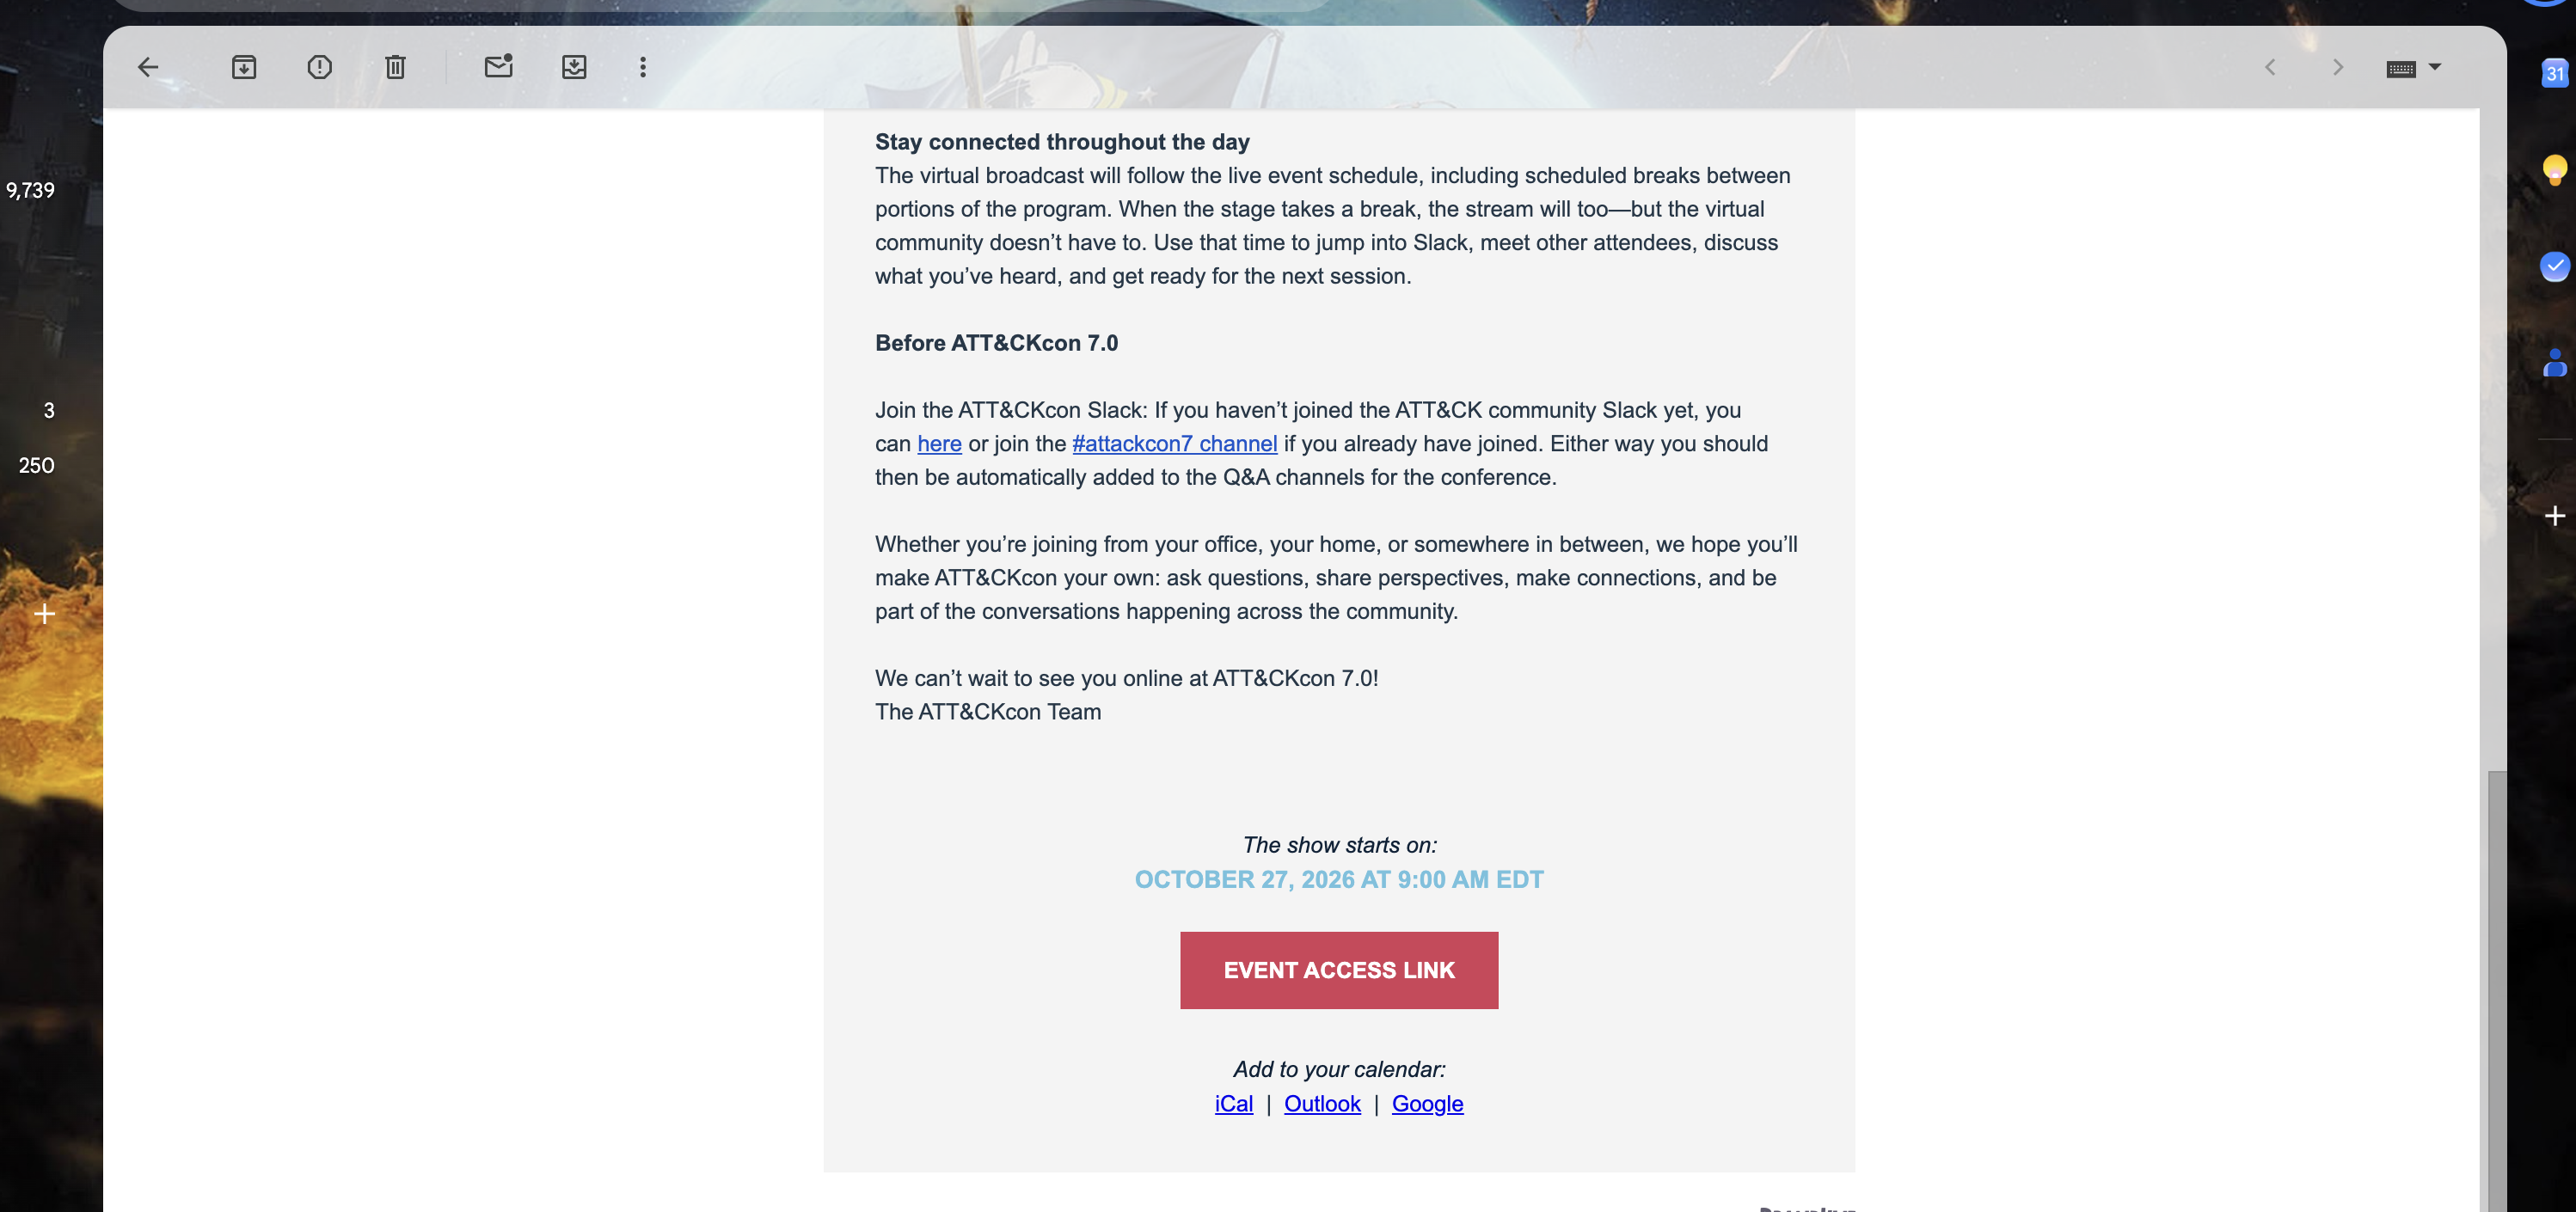
\includegraphics[width=0.58\textwidth,trim=475.02bp 25.00bp 408.02bp 60.00bp,clip]{img/image2.png}
    \caption{Informacion para el acceso virtual al evento.}
\end{figure}


\begin{figure}[H]
    \centering
    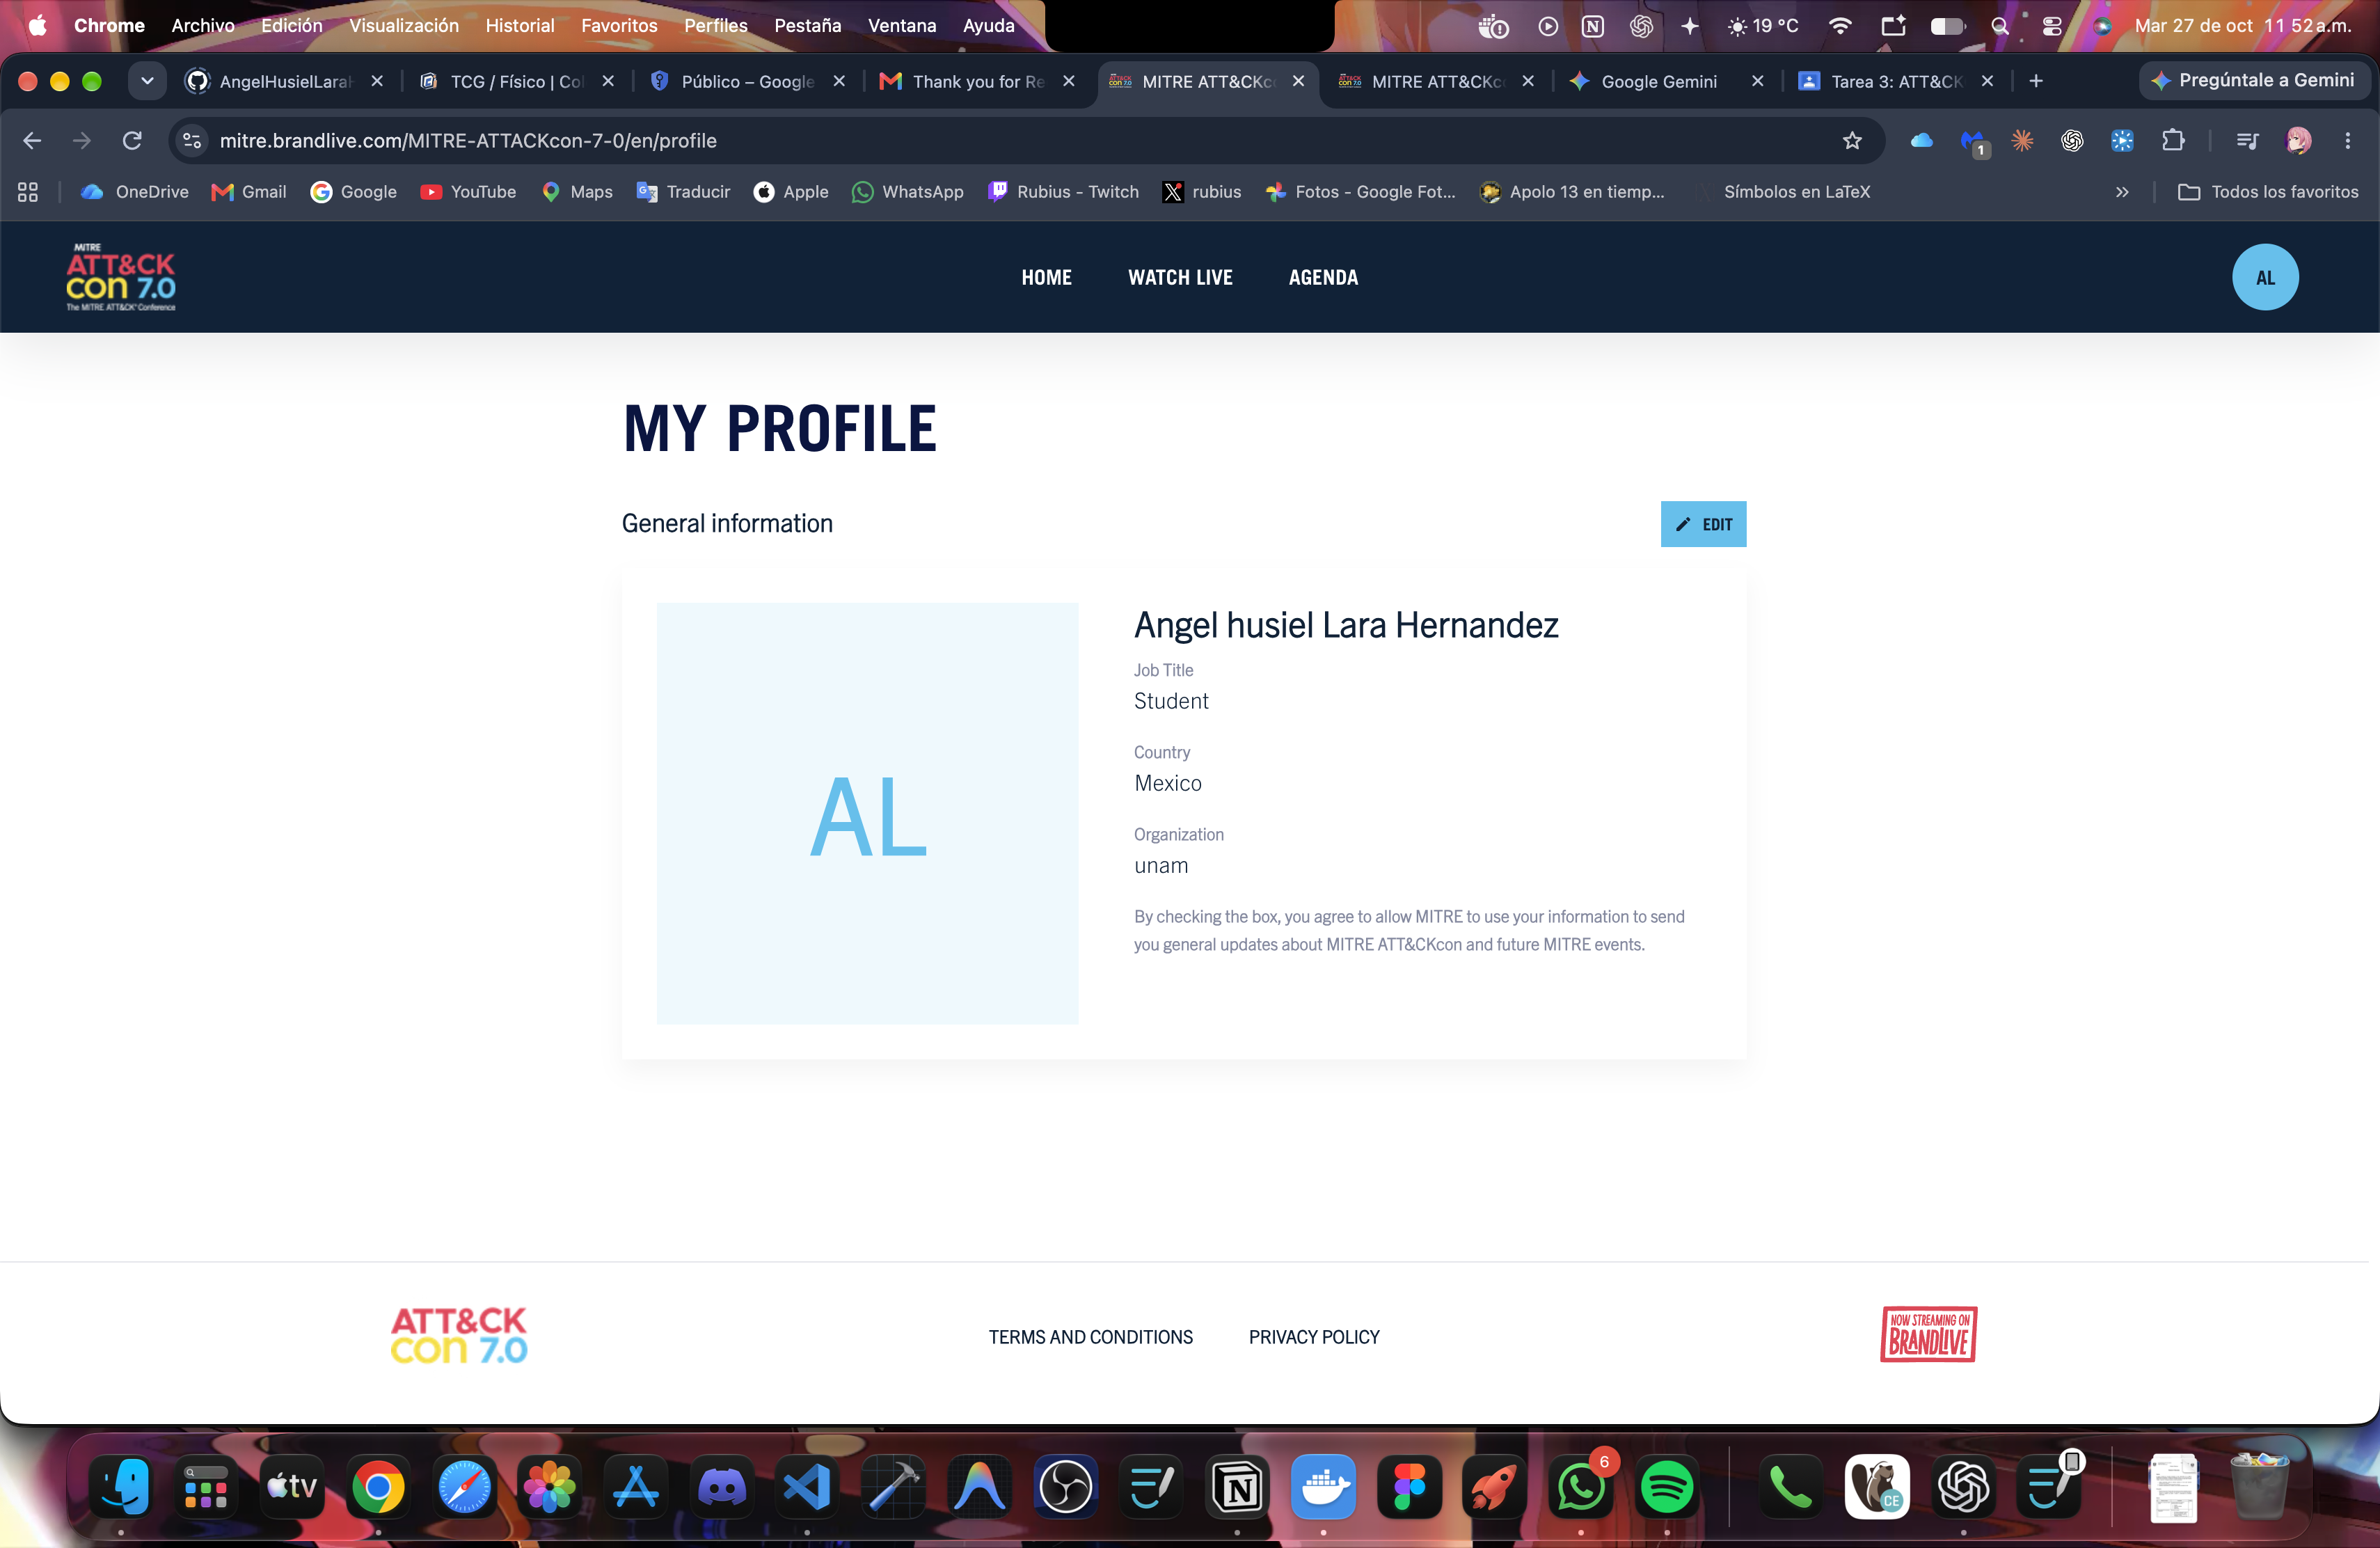
\includegraphics[width=0.63\textwidth,trim=425.02bp 262.01bp 350.02bp 270.01bp,clip]{img/image12.png}
    \caption{Perfil de participante dentro de la plataforma del evento.}
\end{figure}

\newpage
\nocite{*}
\printbibliography[heading=bibintoc,title={Referencias}]
\end{document}
